\documentclass[11pt,a4paper]{article}
\newcommand{\gls}[1]{#1\textsubscript{G}}
\usepackage[utf8]{inputenc}
\usepackage[italian]{babel}
\usepackage{geometry}
\usepackage{graphicx}
\usepackage{float}
\usepackage{tabularx}
\usepackage{booktabs}
\usepackage{caption}
\usepackage{hyperref}
\usepackage{fancyhdr}
\usepackage{lastpage}
\usepackage{longtable}
\usepackage{amsmath}
\usepackage{enumitem}

\usepackage{array}
\newcolumntype{M}[1]{>{\centering\arraybackslash}m{#1}}

\geometry{margin=2.5cm}

% Intestazione e piè di pagina
\pagestyle{fancy}
\fancyhf{}
\renewcommand{\headrulewidth}{0pt}
\fancyfoot[C]{\thepage\ di \pageref{LastPage}}

\begin{document}

% Prima pagina - Intestazione
\begin{titlepage}
    \centering
    
    % Logo Università
    \begin{figure}[H]
        \centering
        
\includegraphics[width=0.3\textwidth]{../logoUnipd.jpg}
    \end{figure}
    
    \vspace{0.5cm}
    
    \textbf{\Large Università degli Studi di Padova} \\
    \vspace{0.2cm}
    \textbf{Laurea in Informatica} \\
    \vspace{0.2cm}
    \textbf{Corso di Ingegneria del Software} \\
    \vspace{0.2cm}
    \textbf{Anno Accademico 2025/2026} \\
    
    \vspace{1cm}
    
    % Logo gruppo
    \begin{figure}[H]
        \centering
        
\includegraphics[width=0.2\textwidth]{../LogoByteMe.jpg}
    \end{figure}
    
    \vspace{0.5cm}
    
    \textbf{\Large Gruppo ByteMe} \\
    \vspace{0.2cm}
    \texttt{byteme2025swe@gmail.com} \\
    
    \vspace{1cm}
    
    \textbf{\Huge \gls{Specifica Tecnica}} \\
    
    \vspace{1.5cm}
    
    \begin{table}[H]
        \centering
        \begin{tabular}{|l|p{5cm}|}
            \hline
            \textbf{Versione} & 0.2.5 \\
            \hline
            \textbf{Stato} & In corso \\
            \hline
            \textbf{Redazione} & Tutto il gruppo\\
            \hline
            \textbf{\gls{Verifica}} & Da verificare\\
            \hline
            \textbf{Approvazione} & Da approvare\\
            \hline
            \textbf{Proprietario} & ByteMe \\
            \hline
            \textbf{Uso} & Esterno \\
            \hline
            \textbf{Destinatari} & Prof. Tullio Vardanega \\ & Prof. Riccardo Cardin \\
            \hline
        \end{tabular}
    \end{table}
    
    \vfill
\end{titlepage}

% Seconda pagina - Versionamento
\thispagestyle{empty}
\section*{Registro dei Cambiamenti}

\begin{longtable}{|>{\centering\arraybackslash}p{0.10\textwidth}|>{\centering\arraybackslash}p{0.12\textwidth}|>{\centering\arraybackslash}p{0.18\textwidth}|>{\raggedright\arraybackslash}p{0.35\textwidth}|>{\raggedright\arraybackslash}p{0.15\textwidth}|}
    \hline
    \textbf{Versione} & \textbf{Data} & \textbf{Autore} & \textbf{Descrizione} & \textbf{\gls{Verifica}} \\
    \hline
    \endhead
        0.2.5 & 29/04/2026 & Elisa Marchioro & Sistemata sezione design pattern frontend & \\
        \hline
        0.2.4 & 29/04/2026 & Matteo Cuogo & Sistemazione layered architecture & Giulia Barzon\\
        \hline
        0.2.3 & 29/04/2026 & Joseph Grant & Aggiunta diagrammi hook, correzione diagrammi & Matteo Cuogo\\
        \hline
        0.2.2 & 26/04/2026 & Giulia Barzon & Aggiornati diagrammi frontend & Joseph Grant \\
        \hline
        0.2.1 & 25/04/2026 & Giulia Barzon & Aggiornamento requisiti soddisfatti & Joseph Grant \\
        \hline
        0.2.0 & 25/04/2026 & Elisa Marchioro & Aggiornamento subsubsection caching & Joseph Grant, Giulia Barzon \\
        \hline
        0.1.9 & 24/04/2026 & Matteo Cuogo & Aggiornamento dello stato di soddisfacimento di alcuni requisiti & Giulia Barzon\\
        \hline
        0.1.8 & 24/04/2026 & Tommaso Tombacco & Modifica sezione AiWidget e modifica dello stato dei requisiti legati ad AI & Giulia Barzon \\
        \hline
        0.1.7 & 23/04/2026 & Giulia Barzon & Aggiunte componenti AI, migliorata sezione 3 & \\
        \hline
        0.1.6 & 23/04/2026 & Elisa Marchioro & Sistemata formattazione, aggiunta sezione \gls{API} e aggiunta diagrammi UML backend & Chiara Grossele \\
        \hline
        0.1.5 & 23/04/2026 & Giulia Barzon & Rivista sezione layered architecture & Elisa Marchioro\\
        \hline
        0.1.4 & 22/04/2026 & Giulia Barzon & Rivista sezione backend e strategy & Elisa Marchioro\\
        \hline
        0.1.3 & 22/04/2026 & Giulia Barzon & Correzione e diagramma sezione Facade, rivisto MVVM & Elisa Marchioro\\
        \hline
        0.1.2 & 22/04/2026 & Elisa Marchioro & Sistemata sezione architettura del backend & Giulia Barzon, Matteo Cuogo\\
        \hline
        0.1.1 & 21/04/2026 & Giulia Barzon & Struttura documento e sezione MVVM, bozza del Facade & Chiara Grossele, Elisa Marchioro\\
        \hline
        0.1.0 & 21/04/2026 & Giulia Barzon & Completate sezione 1, 2 e 3 & Chiara Grossele, Elisa Marchioro\\
        \hline
        0.0.10 & 20/04/2026 & Elisa Marchioro & Fix alle tabelle & Giulia Barzon\\
        \hline
        0.0.9 & 20/04/2026 & Giulia Barzon & Mappatura requisiti soddisfatti (una parte) & Elisa Marchioro\\
        \hline
        0.0.8 & 18/04/2026 & Joseph Grant & Aggiunti i hook frontend & Elisa Marchioro\\
        \hline
        0.0.7 & 18/04/2026 & Matteo Cuogo & Aggiunto operation mapper & Giulia Barzon, Elisa Marchioro\\
        \hline
        0.0.6 & 17/04/2026 & Matteo Cuogo & Aggiunta sezione Design Pattern & Giulia Barzon, Elisa Marchioro\\
        \hline
        0.0.5 & 17/04/2026 & Chiara Grossele & Aggiunta sezione Tracciamento dei requisiti & Matteo Cuogo, Elisa Marchioro\\
        \hline
        0.0.4 & 17/04/2026 & Joseph Grant & Aggiunta descrizione delle componenti frontend & Chiara Grossele, Matteo Cuogo\\
        \hline
        0.0.3 & 15/04/2026 & Chiara Grossele & Modifica struttura e aggiunte alla sezione Architettura backend & Joseph Grant, Matteo Cuogo, Giulia Barzon \\
        \hline
        0.0.2 & 14/04/2026 & Joseph Grant & Aggiunta tecnologie e architettura & Chiara Grossele, Giulia Barzon\\
        \hline
        0.0.1 & 28/03/2026 & Giulia Barzon & Creazione del documento, scrittura introduzione & Tommaso Tombacco \\
        \hline
    \caption{Registro delle versioni del documento}
    \label{tab:versionamento}
\end{longtable}

\newpage

% Terza pagina - Indice
\tableofcontents
\thispagestyle{empty}
\newpage

% indice delle figure = diagrammi
\phantomsection 
\addcontentsline{toc}{section}{Elenco delle Figure} 
\listoffigures 
\newpage

% Contenuto principale
\setcounter{page}{1}

\section{Introduzione}
\subsection{Scopo del documento}
Il presente documento costituisce la \textbf{\gls{Specifica Tecnica}} del prodotto \textit{Second Brain}, proposto dall'azienda \textit{Zucchetti} al gruppo ByteMe.
 
Il documento descrive in dettaglio:
\begin{itemize}
  \item le \textbf{tecnologie} adottate (linguaggi, framework, librerie, strumenti);
  \item l'\textbf{architettura} logica e fisica del sistema, con i pattern architetturali scelti;
  \item i \textbf{design pattern} applicati a livello di componenti, con motivazione delle scelte;
  \item la \textbf{documentazione \gls{API}} tra frontend e backend;
  \item i \textbf{requisiti soddisfatti} con riferimento al documento \textit{\gls{Analisi dei Requisiti}} v2.0.0.
\end{itemize}
 
Il documento è rivolto al team di sviluppo come guida implementativa e a
committente e proponente come \gls{verifica} della coerenza tra scelte progettuali e requisiti concordati.
 
\subsection{Approccio alla redazione}
Il documento viene redatto in modo \textbf{incrementale}, assicurando coerenza con gli sviluppi in corso. Non può essere considerato completo fino al rilascio della versione 1.0.0.

\subsection{Scopo del prodotto}
Il progetto \textit{Second Brain} mira a sviluppare un \gls{editor di testo} avanzato basato sul linguaggio \gls{Markdown} e potenziato dall'integrazione di Large Language Model (LLM).
L'applicazione web consentirà all'utente di:
\begin{itemize}
  \item scrivere e visualizzare in tempo reale testi formattati in \gls{Markdown};
  \item interagire con un LLM per riassumere, correggere, riscrivere e tradurre testi;
  \item ottenere analisi critiche multi-prospettiche secondo il metodo dei \textit{Sei Cappelli per Pensare} di Edward De Bono;
  \item delegare all'AI la stesura completa di un testo tramite \gls{Distant Writing}.
\end{itemize}
 
\subsection{\gls{Glossario}}
Per evitare ambiguità, i termini tecnici usati nel documento vengono definiti in modo più approfondito nel documento \gls{Glossario} v2.0.0 che si può trovare nel sito web del gruppo ByteMe alla sezione Documenti Interni e raggiungibile dal seguente link:\\
\href{https://byteme25.github.io/ByteMe/files.html}{ByteMe/\gls{Glossario} v2.0.0}

I termini che vengono considerati meritevoli di approfondimenti sono indicati con una G a pedice.


\subsection{Riferimenti}
\begin{itemize}
  \item \textit{\gls{Norme di Progetto}} versione 2.0.0 (Ultimo accesso: 20/04/2026)\\
  \href{https://byteme25.github.io/ByteMe/files.html}{ByteMe/\gls{Norme di Progetto} v2.0.0}
  \item Capitolato d'appalto C6: \textit{Second Brain} (Zucchetti S.p.A.)\\ \url{https://www.math.unipd.it/~tullio/IS-1/2025/Progetto/C6.pdf}
  \item Regolamento del progetto didattico:\\
        \url{https://www.math.unipd.it/~tullio/IS-1/2023/Dispense/PD2.pdf}
\end{itemize}
 
\subsubsection{Riferimenti informativi}
\begin{itemize}
    \item \textit{\gls{Analisi dei Requisiti}} versione 2.0.0 (Ultimo accesso: 20/04/2026)\\
    \href{https://byteme25.github.io/ByteMe/}{PB - \gls{Analisi dei Requisiti} v2.0.0}
    \item \textit{Piano di Qualifica} versione 2.0.0 (Ultimo accesso: 20/04/2026) \\
    \href{https://byteme25.github.io/ByteMe/}{PB - Piano di Qualifica v2.0.0}
    \item Verbali interni ed esterni
    \item \gls{Glossario} versione 2.0.0 (Ultimo accesso: 20/04/2026)\\
    \href{https://byteme25.github.io/ByteMe/files.html}{Documenti interni - \gls{Glossario} v2.0.0}
    \item \gls{Repository} ufficiale di \gls{EasyMDE}: \url{https://github.com/Ionaru/easy-markdown-editor}\\ (Ultimo accesso: 24/03/2026)
     \item Documentazione linguaggio \gls{markdown} - CommonMark: \url{https://commonmark.org/}\\ (Ultimo accesso: 20/02/2026)
    \item Documentazione \gls{React} 19: \url{https://react.dev}\\ (Ultimo accesso: 16/04/2026)
    \item Principi del Bulletproof \gls{React} (\gls{repository} ufficiale): \url{https://github.com/alan2207/bulletproof-react}\\ (Ultimo accesso: 16/04/2026)
    \item Documentazione \gls{Flask}: \url{https://flask.palletsprojects.com}\\ (Ultimo accesso: 10/03/2026)
    \item Documentazione \gls{Docker}: \url{https://docs.docker.com}\\ (Ultimo accesso: 27/02/2026)
    \item Documentazione TypeScript: \url{https://www.typescriptlang.org/docs/}\\ (Ultimo accesso: 27/03/2026)

    \item Slide del corso di Ingegneria del Software\\ (Ultimo accesso: 10/04/2026)
    \item Principi SOLID (slide prof. Cardin)
    \item Pattern architetturali (slide prof. Cardin)
\end{itemize}

\newpage

\section{Tecnologie}
\subsection{Framework frontend}
\begin{table}[H]
    \centering
    \begin{tabular}{|p{0.20\textwidth}|p{0.10\textwidth}|p{0.55\textwidth}|}
        \hline
        \textbf{Nome} & \textbf{Versione} & \textbf{Descrizione} \\
        \hline
        \gls{React} & 19.2.0 & Libreria JavaScript per la costruzione di interfacce utente basate su componenti riutilizzabili. \\
        \hline
    \end{tabular}
    \caption{Descrizione del framework frontend}
    \label{tab:framework_frontend}
\end{table}

\subsection{Librerie frontend}
\begin{table}[H]
    \centering
    \begin{tabular}{|p{0.20\textwidth}|p{0.10\textwidth}|p{0.55\textwidth}|}
        \hline
        \textbf{Nome} & \textbf{Versione} & \textbf{Descrizione} \\
        \hline
        \gls{EasyMDE} & 2.20.0 & Editor \gls{Markdown} con anteprima in tempo reale, basato su CodeMirror. \\
        \hline
        Axios & 1.7.9 & Client HTTP basato su Promise per effettuare richieste REST dal browser. \\
        \hline
        \gls{React Router} DOM & 7.13.1 & Libreria standard per il routing dichiarativo in applicazioni \gls{React}, utilizzata per la navigazione tra le viste. \\
        \hline
        \gls{Zustand} & 5.0.12 & Libreria di state management leggera, utilizzata per la gestione dello stato globale e la persistenza dei dati nel LocalStorage. \\
        \hline
        Lucide-\gls{React} & 1.8.0 & Libreria di icone vettoriali utilizzata per la UI dell'applicazione. \\
        \hline
        \gls{React} Hot Toast & 2.6.0 & Libreria leggera per la visualizzazione di notifiche toast personalizzabili. \\
        \hline
        \gls{CSS Modules} & N/A (Integrato) & Sistema di scope locale per i fogli di stile CSS integrato in \gls{Vite}, che evita conflitti tra classi. \\
        \hline
        ESLint & 9.39.1 & Strumento di linting per TypeScript, che aiuta a mantenere uno stile di codice coerente e a individuare errori. \\
        \hline
    \end{tabular}
    \caption{Descrizione delle librerie frontend}
    \label{tab:librerie_frontend}
\end{table}

\subsection{Linguaggio frontend}
\begin{table}[H]
    \centering
    \begin{tabular}{|p{0.20\textwidth}|p{0.10\textwidth}|p{0.55\textwidth}|}
        \hline
        \textbf{Nome} & \textbf{Versione} & \textbf{Descrizione} \\
        \hline
        TypeScript & 5.9.3 & Superset tipizzato di JavaScript che aggiunge tipizzazione statica e migliora la manutenibilità del codice. \\
        \hline
        TSX & N/A (Sintassi) & Estensione di TypeScript che consente di scrivere markup \gls{JSX} all'interno di file tipizzati, usata per i componenti \gls{React}. \\
        \hline
    \end{tabular}
    \caption{Descrizione dei linguaggi frontend}
    \label{tab:linguaggi_frontend}
\end{table}

\subsection{Tecnologie di build e runtime}
\begin{table}[H]
    \centering
    \begin{tabular}{|p{0.20\textwidth}|p{0.10\textwidth}|p{0.55\textwidth}|}
        \hline
        \textbf{Nome} & \textbf{Versione} & \textbf{Descrizione} \\
        \hline
        \gls{Vite} & 7.3.1 & Build tool moderno e veloce per applicazioni web, con supporto nativo a ES modules e Hot Module Replacement. \\
        \hline
        Node.js & 20-alpine & Ambiente di runtime JavaScript lato server, utilizzato nel \gls{Dockerfile} per la fase di compilazione del frontend. \\
        \hline
    \end{tabular}
    \caption{Descrizione delle tecnologie di build}
    \label{tab:tecnologie_build}
\end{table}

\subsection{Tecnologie di test}
\begin{table}[H]
    \centering
    \begin{tabular}{|p{0.20\textwidth}|p{0.10\textwidth}|p{0.55\textwidth}|}
        \hline
        \textbf{Nome} & \textbf{Versione} & \textbf{Descrizione} \\
        \hline
        \gls{Vitest} & 4.1.4 & Framework di testing per applicazioni \gls{Vite}, compatibile con l'\gls{API} di Jest e ottimizzato per TypeScript. \\
        \hline
        \gls{Pytest} & 7.0.0 & Framework di testing per Python, con sintassi semplice e supporto a fixture, parametrizzazione e plugin. \\
        \hline
        \gls{React} testing library & 16.3.2 & Libreria per il testing di componenti \gls{React}, che fornisce utilities per interagire con i componenti in modo simile a come un utente reale lo farebbe. \\
        \hline
    \end{tabular}
    \caption{Descrizione delle tecnologie di test}
    \label{tab:tecnologie_test}
\end{table}

\subsection{Framework \gls{API} backend}
\begin{table}[H]
    \centering
    \begin{tabular}{|p{0.20\textwidth}|p{0.10\textwidth}|p{0.55\textwidth}|}
        \hline
        \textbf{Nome} & \textbf{Versione} & \textbf{Descrizione} \\
        \hline
        \gls{Flask} & 3.1.3 & Microframework Python per lo sviluppo di \gls{API} REST, leggero ed estensibile tramite plugin. \\
        \hline
    \end{tabular}
    \caption{Descrizione del framework \gls{API} backend}
    \label{tab:api_backend}
\end{table}

\subsection{Linguaggio backend}
\begin{table}[H]
    \centering
    \begin{tabular}{|p{0.20\textwidth}|p{0.10\textwidth}|p{0.55\textwidth}|}
        \hline
        \textbf{Nome} & \textbf{Versione} & \textbf{Descrizione} \\
        \hline
        Python & 3.12-slim & Linguaggio di programmazione ad alto livello, utilizzato per la logica di business e l'implementazione delle \gls{API}. \\
        \hline
    \end{tabular}
    \caption{Descrizione del linguaggio backend}
    \label{tab:linguaggio_backend}
\end{table}

\subsection{Librerie backend}
\begin{table}[H]
    \centering
    \begin{tabular}{|p{0.20\textwidth}|p{0.10\textwidth}|p{0.55\textwidth}|}
        \hline
        \textbf{Nome} & \textbf{Versione} & \textbf{Descrizione} \\
        \hline
        OpenAI & 2.31.0 & Libreria ufficiale utilizzata per l'integrazione e la comunicazione con le \gls{API} dei modelli linguistici (LLM). \\
        \hline
        Pydantic & 2.12.5 & Libreria per la \gls{validazione} dei dati e la serializzazione tramite annotazioni di tipo nativo in Python. \\
        \hline
        \gls{Flask}-CORS & 6.0.2 & Estensione di \gls{Flask} per la gestione sicura del Cross-Origin Resource Sharing tra frontend e backend. \\
        \hline
        Python-dotenv & 1.2.2 & Modulo per il caricamento delle variabili d'ambiente e chiavi \gls{API} dai file \texttt{.env}. \\
        \hline
        lru-cache & 11.3.5 & Libreria per implementare una cache in memoria con politica di rimozione LRU (Least Recently Used). \\
        \hline
    \end{tabular}
    \caption{Descrizione delle librerie backend}
    \label{tab:librerie_backend}
\end{table}

\subsection{Server Web}
\begin{table}[H]
    \centering
    \begin{tabular}{|p{0.20\textwidth}|p{0.10\textwidth}|p{0.55\textwidth}|}
        \hline
        \textbf{Nome} & \textbf{Versione} & \textbf{Descrizione} \\
        \hline
        \gls{Nginx} & alpine & Server web ad alte prestazioni utilizzato nel container \gls{Docker} per servire i file statici del frontend e gestire il routing. \\
        \hline
        Werkzeug & 3.1.8 & Server WSGI integrato in \gls{Flask}, utilizzato attualmente come motore di esecuzione per l'ambiente backend. \\
        \hline
    \end{tabular}
    \caption{Descrizione dei server web frontend e backend}
    \label{tab:server_web}
\end{table}

\subsection{Tecnologie deployment}
\begin{table}[H]
    \centering
    \begin{tabular}{|p{0.20\textwidth}|p{0.10\textwidth}|p{0.55\textwidth}|}
        \hline
        \textbf{Nome} & \textbf{Versione} & \textbf{Descrizione} \\
        \hline
        \gls{Docker} & 29.4.0 & Piattaforma per la containerizzazione, utilizzata per isolare frontend e backend in ambienti riproducibili. \\
        \hline
        \gls{Docker Compose} & 5.1.2 & Strumento per definire e gestire applicazioni multi-container tramite il file \texttt{\gls{docker}-compose.yml}. \\
        \hline
    \end{tabular}
    \caption{Descrizione delle tecnologie di deployment}
    \label{tab:tecnologie_deployment}
\end{table}

\newpage

\section{Architettura di deployment}
Il sistema \textit{Second Brain} si basa su un'architettura di deployment di tipo \textbf{Client-Server}, distribuita fisicamente su nodi (container) logici distinti. Per l'implementazione pratica, il progetto utilizza la tecnologia di containerizzazione \textbf{\gls{Docker}} per garantire l'isolamento dei componenti, la portabilità tra diversi ambienti di sviluppo o produzione e la gestione semplificata delle dipendenze.

\subsection{Strategia di containerizzazione}
L'applicativo è suddiviso in due servizi principali (il nodo Client e il nodo Server) orchestrati tramite \texttt{\gls{docker}-compose}. Questo strumento permette di definire reti virtuali interne, gestire le variabili d'ambiente in modo centralizzato e montare volumi per l'\textit{hot-reloading} durante le fasi di sviluppo.

\subsection{Backend (\gls{Flask})}
Il container del backend agisce da Server ed è ottimizzato per l'esecuzione del codice Python in un ambiente leggero e sicuro.
\begin{itemize}
    \item \textbf{Immagine di base}: \texttt{python:3.12-slim}. La scelta della variante \textit{slim} riduce l'ingombro dell'immagine base, contenendo solo le librerie di sistema essenziali per il runtime Python 3.12.
    \item \textbf{Configurazione}: La directory di lavoro (\texttt{WORKDIR}) è impostata su \texttt{/app}. Il sistema installa le dipendenze tramite \texttt{pip} utilizzando il flag \texttt{--no-cache-dir} per mantenere l'immagine di produzione più snella.
    \item \textbf{Networking e Sicurezza}: Il container espone internamente la porta \texttt{8000}. Il backend riceve dinamicamente (tramite il file \texttt{.env} mappato nel Compose) le chiavi segrete e le credenziali per l'accesso ai provider LLM, evitando di esporre dati sensibili nel codice sorgente.
\end{itemize}

\subsection{Frontend (\gls{React} + \gls{Nginx})}
Il container del frontend agisce da nodo Client. Per la sua realizzazione è stata adottata una strategia di \textbf{Multi-stage Build}, che separa l'ambiente di compilazione da quello di esecuzione per minimizzare la dimensione finale dell'immagine.
\begin{itemize}
    \item \textbf{Stage 1 (Build)}: Utilizza \texttt{node:20-alpine} per installare le dipendenze ed eseguire la build di produzione (\texttt{npm run build}) tramite \gls{Vite}. L'uso di Alpine Linux garantisce velocità nel processo di CI/CD.
    \item \textbf{Stage 2 (Production)}: I file statici generati dalla build (\texttt{dist}) vengono copiati in un'immagine \texttt{\gls{nginx}:alpine}. \gls{Nginx} funge da web server statico ad alte prestazioni. Un aspetto cruciale di questo livello è l'iniezione di un file di configurazione personalizzato (\texttt{\gls{nginx}.conf}), necessario per indirizzare tutte le richieste al file \texttt{index.html} e gestire correttamente il routing \textit{client-side} della Single Page Application (SPA).
\end{itemize}

\subsection{Orchestrazione: \gls{Docker Compose}}
Il file \texttt{\gls{docker}-compose.yml} coordina l'avvio sincronizzato dei servizi e la gestione delle risorse:
\begin{itemize}
    \item \textbf{Mapping delle porte}: Il frontend è reso accessibile all'host esterno sulla porta \texttt{8080}, mappata sulla porta interna \texttt{80} del server \gls{Nginx}.
    \item \textbf{Dipendenze di avvio}: È definita una clausola \texttt{depends\_on} che assicura che il container del backend sia istanziato prima di quello del frontend. Inoltre, la direttiva \texttt{pull\_policy: never} protegge l'ambiente di sviluppo dal download accidentale di immagini omonime dai registri pubblici.
    \item \textbf{Ottimizzazione per lo sviluppo (Hot-reloading)}: Per velocizzare il ciclo di sviluppo, viene configurato un \textit{bind mount} (\texttt{./backend/src:/app/backend/src}) che permette al server \gls{Flask} di riflettere istantaneamente le modifiche al codice sorgente senza dover ricostruire l'immagine del container a ogni salvataggio.
    \item \textbf{Iniezione dell'ambiente}: Il Compose si occupa di orchestrare e iniettare dinamicamente le variabili di configurazione (\texttt{environment}), prelevando le chiavi \gls{api} dei modelli LLM e i \textit{secret} applicativi direttamente dall'host, mantenendo i container agnostici rispetto alle credenziali.
\end{itemize}

% immagine rappresentativa dell'ambiente docker
\begin{figure}[H]
    \centering
    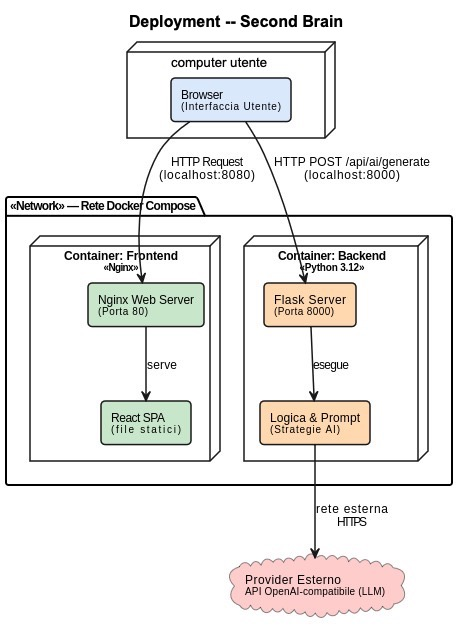
\includegraphics[width=0.9\textwidth]{../UMLimg/imgDocker.jpg}
    \caption{Rappresentazione dell'architettura di deployment tramite \gls{Docker Compose}}
    \label{fig:architettura_deployment}
\end{figure}



\newpage

\section{\gls{API}}
Il sistema adotta un’architettura basata su \gls{API} REST (Representational State Transfer), uno stile architetturale per servizi web che consente comunicazione standardizzata, scalabile e disaccoppiata tra client e server. REST si basa sull’utilizzo del protocollo HTTP e sull’identificazione delle risorse tramite URI, promuovendo semplicità, interoperabilità e manutenibilità.

\subsection{Principi e requisiti delle \gls{API} REST}
Per essere conforme allo stile REST, il sistema rispetta i seguenti principi:
\begin{itemize}
\item \textbf{Architettura client-server}: separazione netta tra frontend e backend;
\item \textbf{Statelessness}: ogni richiesta contiene tutte le informazioni necessarie per essere elaborata e il server non mantiene stato tra richieste successive.
\item \textbf{Interfaccia uniforme}: utilizzo coerente di:
    \begin{itemize}[label=\textbullet]
        \item URI per identificare le risorse;
        \item Metodi HTTP standard:
            GET → recupero dati;
            POST → creazione/elaborazione;
            PUT/PATCH → aggiornamento;
            DELETE → rimozione.
\end{itemize}
\item \textbf{Formato dei dati standardizzato}: scambio dati in formato JSON, facilmente leggibile e interoperabile tra sistemi eterogenei.
\item \textbf{Separazione delle responsabilità (\gls{Separation of Concerns})}: il client gestisce la presentazione, il server gestisce logica, orchestrazione e integrazione con servizi esterni.
\item \textbf{Scalabilità}: grazie alla natura \gls{stateless}, il backend può essere replicato e distribuito senza gestione di sessioni condivise.
\end{itemize}

\subsection{Comunicazione client–server (Axios)}
Nel frontend, la comunicazione con le \gls{API} REST avviene tramite la libreria \textbf{Axios}, un HTTP client basato su promise che semplifica l’invio di richieste asincrone e la gestione delle risposte. 
Nel contesto dell’applicazione, Axios è utilizzato nel frontend come client HTTP centralizzato per invocare le \gls{API} REST esposte dal backend. In particolare, gestisce l’interazione con l’\gls{endpoint} di generazione AI (POST /\gls{api}/ai/generate), incapsulando tutta la logica di comunicazione.

Nel dettaglio, Axios svolge le seguenti funzioni:
\begin{itemize}
\item \textbf{Invio delle richieste al backend}:
Costruisce e invia la richiesta POST verso l’\gls{endpoint} /\gls{api}/ai/generate contenente:
\begin{itemize}[label=\textbullet]
\item il testo inserito dall’utente (text);
\item l’operazione richiesta (operation);
\end{itemize}

\item \textbf{Gestione asincrona della comunicazione}: permette al frontend di utilizzare async/await per gestire la chiamata senza bloccare l’interfaccia utente, migliorando la user experience.
\item \textbf{Serializzazione automatica dei dati}: converte automaticamente gli oggetti JavaScript in JSON per il body della richiesta, senza necessità di gestione manuale.
\item \textbf{Gestione della risposta}: riceve il JSON dal backend (es. generated\_text) e lo rende immediatamente disponibile al frontend per l’aggiornamento della UI.
\item \textbf{Gestione degli errori}: centralizza la gestione di errori HTTP o di rete (es. 400, 500), permettendo di definire comportamenti uniformi (messaggi utente, retry, logging).
\item \textbf{Configurazione condivisa}: consente di definire in un unico punto:
\begin{itemize}[label=\textbullet]
\item baseURL del backend;
\item eventuali headers;
\item timeout e policy di retry.
\end{itemize}
\end{itemize}

\subsection{Flusso di elaborazione}
\begin{enumerate}
\item Il frontend invia una richiesta HTTP POST tramite Axios.
\item Il controller backend riceve la richiesta e valida i dati.
\item Viene selezionata la strategia di elaborazione tramite un registry interno.
\item Il sistema costruisce i \gls{prompt} per il modello AI.
\item Il backend invoca il modello per generare il contenuto.
\item La risposta viene pulita e normalizzata.
\item Il risultato viene restituito al client in formato JSON e gestito dal frontend.
\end{enumerate}


\newpage

% architettura di sistema (generale)
\section{Architettura del sistema}
\subsection{Layered Architecture}
Il sistema \textit{Second Brain} è stato progettato adottando il pattern architetturale \textbf{Layered Architecture} (o Architettura a Livelli), considerato lo standard \textit{de facto} per lo sviluppo di applicazioni moderne e scalabili.

Il principio cardine di questo pattern è la \textbf{\gls{Separation of Concerns}} (Separazione delle Responsabilità): i componenti del sistema sono organizzati in strati orizzontali, dove ogni strato fornisce un'astrazione specifica e gestisce esclusivamente la logica di propria competenza. Questo approccio modulare limita il raggio d'azione dei singoli componenti, semplificando notevolmente lo sviluppo, il testing e la manutenzione dell'applicazione.

\paragraph{Vincolo dei "Closed Layers" (Strati Chiusi)}
Una caratteristica fondamentale di un'architettura a livelli ben progettata è l'isolamento degli strati. Affinché l'architettura sia solida, gli strati devono essere \textbf{chiusi}. Questo significa che il flusso di esecuzione segue una direttiva strettamente \textit{top-down}: una richiesta può transitare esclusivamente allo strato immediatamente sottostante. Di conseguenza, i livelli superiori ignorano del tutto i dettagli implementativi dei livelli inferiori, garantendo che le modifiche effettuate all'interno di uno strato non generino impatti a cascata sugli altri.

L'implementazione standard adottata prevede la scomposizione del sistema in tre livelli logici:
\begin{itemize}
    \item \textbf{Presentation Layer}: Responsabile della gestione dell'interfaccia utente.
    \item \textbf{Application Logic}: Riceve le informazioni dall'esterno, effettua i controlli formali, orchestra le operazioni e gestisce il flusso applicativo.
    \item \textbf{Business Logic}: Il cuore del sistema, che implementa la logica funzionale vera e propria e le regole di dominio, isolato dal sistema di rete.
\end{itemize}    

\subsection{Applicazione del pattern in "Second Brain"}
Di seguito viene descritto in dettaglio come i moduli e i file del progetto realizzano i tre livelli teorici dell'architettura.


\subsubsection{Presentation Layer}
Questo strato è fisicamente e logicamente disaccoppiato dal backend. È interamente delegato all'applicativo \textbf{Frontend} sviluppato in \gls{React} e \gls{TypeScript}. Non esegue elaborazioni semantiche sui testi, ma si occupa esclusivamente di presentare l'interfaccia visiva (UI), raccogliere gli input dell'utente (testo, preferenze di formattazione o di intelligenza artificiale) e inoltrare tali richieste al livello sottostante tramite chiamate \gls{api} HTTP.

% ===================
% APPLICATION LOGIC
% ===================
\subsubsection{Application Logic}
L'Application Logic rappresenta il punto di ingresso lato server. Nel sistema, questo ruolo è svolto integralmente dal modulo di routing del framework \gls{Flask} all'interno del file \texttt{app.py}, che agisce a tutti gli effetti come \textbf{Controller} delle \gls{api} HTTP (comunicanti via JSON). Questo strato non contiene logica di dominio né conoscenza della struttura dei \gls{prompt} o dei modelli LLM: si limita a validare i payload in ingresso e a delegare l'elaborazione agli strati sottostanti, intercettando e formattando eventuali eccezioni.

\subsubsection{Modulo: \texttt{app.py}}
Il modulo non adotta una struttura a classi, ma è organizzato come un insieme di funzioni e configurazioni \gls{Flask}.
\begin{itemize}
    \item \texttt{app}: Istanza dell'applicazione \gls{Flask}, configurata con CORS abilitato per permettere la comunicazione sicura col frontend.
    \item \texttt{generate\_ai\_text()}: Funzione principale del modulo, mappata sull'\gls{endpoint} POST \texttt{/\gls{api}/ai/generate}. Riceve il payload JSON, estrae i parametri e agisce da \textit{Gateway}: interroga la mappatura delle operazioni, recupera l'istanza del modello e delega alla Business Logic la costruzione dei \gls{prompt}. Infine, restituisce la risposta elaborata al client. In caso di errore, cattura l'eccezione e restituisce una risposta standardizzata con il messaggio di errore.
    \item \texttt{root()}: Funzione mappata sull'\gls{endpoint} GET \texttt{/}, utilizzata come \textit{health check} per verificare che il server sia attivo. Restituisce lo stato del servizio e la lista delle operazioni supportate.
\end{itemize}


% ===================
% BUSINESS LOGIC
% ===================
\subsubsection{Business Logic}
La \textbf{Business Logic} rappresenta il nucleo funzionale del sistema, completamente isolato dal framework web e dal protocollo HTTP. Questo strato si occupa di orchestrare il flusso dei dati e definire le regole di dominio per la costruzione dei contesti da inviare ai modelli di linguaggio. L'architettura di questo livello è suddivisa in moduli specializzati che utilizzano Design pattern per gestire l'elevata variabilità delle operazioni richieste.

\subsubsection{Modulo: \texttt{ai\_strategies.py} (Gestione dei \gls{prompt})}
Questo modulo contiene la logica di business necessaria per la generazione dinamica dei \gls{prompt}. Definisce i parametri operativi, come la \gls{temperatura}, e le istruzioni esatte per ogni tipo di elaborazione richiesta (editoriale, traduzione o analisi con i Sei Cappelli di De Bono). 

Per gestire l'ampia gamma di operazioni in modo estensibile e modulare, le classi contenute in questo file (come \texttt{SimplePromptStrategy} e \texttt{DeBonoHatStrategy}) implementano il \textbf{Pattern Strategy}. Questo permette di isolare la logica di costruzione del testo di sistema dal resto dell'applicazione.

\textit{Nota}: I dettagli delle singole classi sono approfonditi nella sezione relativa ai Design Pattern.


\subsubsection{Modulo: \texttt{operation\_mapper.py} (Mappatura Operazioni)}
Questo modulo funge da punto di giunzione dell'intera architettura, orchestrando il legame tra le strategie di contenuto (\gls{prompt}) e le strategie di esecuzione (modelli LLM).

\paragraph{Problema}
L’integrazione tra le diverse strategie di prompting e i diversi LLM poneva un problema di accoppiamento rigido e di complessità gestionale. Senza un punto di coordinamento centrale, il Controller (\texttt{app.py}) avrebbe dovuto:
\begin{itemize}
    \item Conoscere l'esistenza di tutte le classi concrete e importarle direttamente.
    \item Gestire manualmente la logica di accoppiamento tra \gls{prompt} e modelli.
    \item Contenere lunghi blocchi condizionali per istanziare la strategia corretta in base alla stringa ricevuta dal frontend.
\end{itemize}
Questa struttura avrebbe violato il principio di Inversione delle Dipendenze, rendendo l'aggiunta di una nuova operazione un processo rischioso e richiedendo la modifica del codice di routing principale ogni volta che viene introdotta una nuova funzionalità. Per ovviare a questo, si è optato per una mappatura centralizzata.

\paragraph{OperationConfig} 
La struttura \texttt{OperationConfig} è definita tramite un \texttt{@dataclass} ed è progettata per garantire un accoppiamento debole tra i componenti. Agisce come un contenitore che incapsula le dipendenze necessarie a ogni singola operazione.
\begin{itemize}
    \item\textbf{Attributi:}
    \begin{itemize}
        \item \texttt{model\_class} (\texttt{Type[AIModelStrategy]}): è il riferimento al tipo della classe del modello da istanziare, la cui creazione effettiva è delegata al sistema di caching (\texttt{get\_model}).
        \item \texttt{\gls{prompt}\_strategy} (\texttt{BaseAIStrategy}): è un'istanza preconfigurata della strategia di \gls{prompt} specifica per quell'operazione.
    \end{itemize}
\end{itemize}


\paragraph{OPERATION\_MAPPER}
Il nucleo del sistema è implementato come un dizionario globale che associa identificatori testuali univoci (es. \texttt{"summary"}, \texttt{"green\_hat"}) a oggetti \texttt{OperationConfig}. Questa architettura garantisce tre proprietà fondamentali:
\begin{itemize}
    \item \textbf{Adesione al principio Open-Closed}: Per aggiungere una nuova funzionalità è sufficiente registrare una nuova riga nel dizionario di configurazione. Il codice del controller rimane del tutto inalterato, chiuso alle modifiche ma aperto alle estensioni.
    \item \textbf{Routing dinamico dei modelli}: Permette di assegnare il modello più adatto a una specifica operazione. Ad esempio, nel sistema le operazioni logiche di pensiero laterale dei Sei Cappelli sono delegate a \gls{Gemma 3:4B}.
    \item \textbf{Robustezza e fallback}: In caso di operazione non riconosciuta o assente nel payload della richiesta, il sistema fornisce una configurazione di default in modo trasparente tramite la costante \texttt{DEFAULT\_OPERATION\_KEY= "summary"}, sfruttando il metodo \texttt{.get()} del dizionario ed evitando crash dell'applicazione.
\end{itemize}


\subsubsection{Modulo: \texttt{model\_strategies.py} (Integrazione LLM)}
Permette l'astrazione della comunicazione con i provider esterni. Le classi contenute in questo file si occupano di iniettare le chiavi \gls{API} lette dall'ambiente e di impacchettare la richiesta nel formato corretto. Anche in questo caso le classi (\texttt{ZucchettiDeepSeekStrategy}, \texttt{Gemma3Strategy}, \texttt{Qwen3Strategy}) implementano il \textbf{Pattern Strategy}.
\begin{itemize}
    \item \textbf{Caching (\texttt{get\_model})}: All'interno di questo modulo è implementata una funzione per l'istanziazione dei modelli LLM. Per evitare di aprire connessioni ridondanti, la funzione è ottimizzata tramite il decoratore \texttt{@lru\_cache} della libreria standard \texttt{functools}. Alla prima richiesta di una classe modello, l'istanza viene creata; alle chiamate successive, il decoratore intercetta la richiesta e restituisce direttamente il riferimento in memoria, garantendo efficienza e sicurezza concorrenziale (thread-safety).
\end{itemize}


\subsubsection{Modulo: \texttt{utils/text\_cleaning.py} (Servizi di supporto)}
Sottomodulo funzionale che utilizza espressioni regolari (regex) per validare e "ripulire" l'output testuale grezzo generato dagli LLM. Il suo scopo è garantire che il testo restituito al client sia privo di metatesto, preamboli discorsivi o tag \gls{markdown} residui, assicurando la coerenza del dominio.

\newpage

% STRATEGY
\section{Backend: design pattern}
La progettazione del backend di \textit{Second Brain} si basa sull'applicazione di design pattern comportamentali e creazionali. L'obiettivo primario di questa scelta architetturale è garantire l'estensibilità del sistema: l'aggiunta di nuove operazioni AI o l'integrazione di nuovi modelli LLM deve poter avvenire senza alterare il codice di routing esistente, nel pieno rispetto dei principi SOLID (in particolare l'\textit{Open-Closed Principle} e il \textit{Single Responsibility Principle}).

\begin{figure}[H]
    \centering
    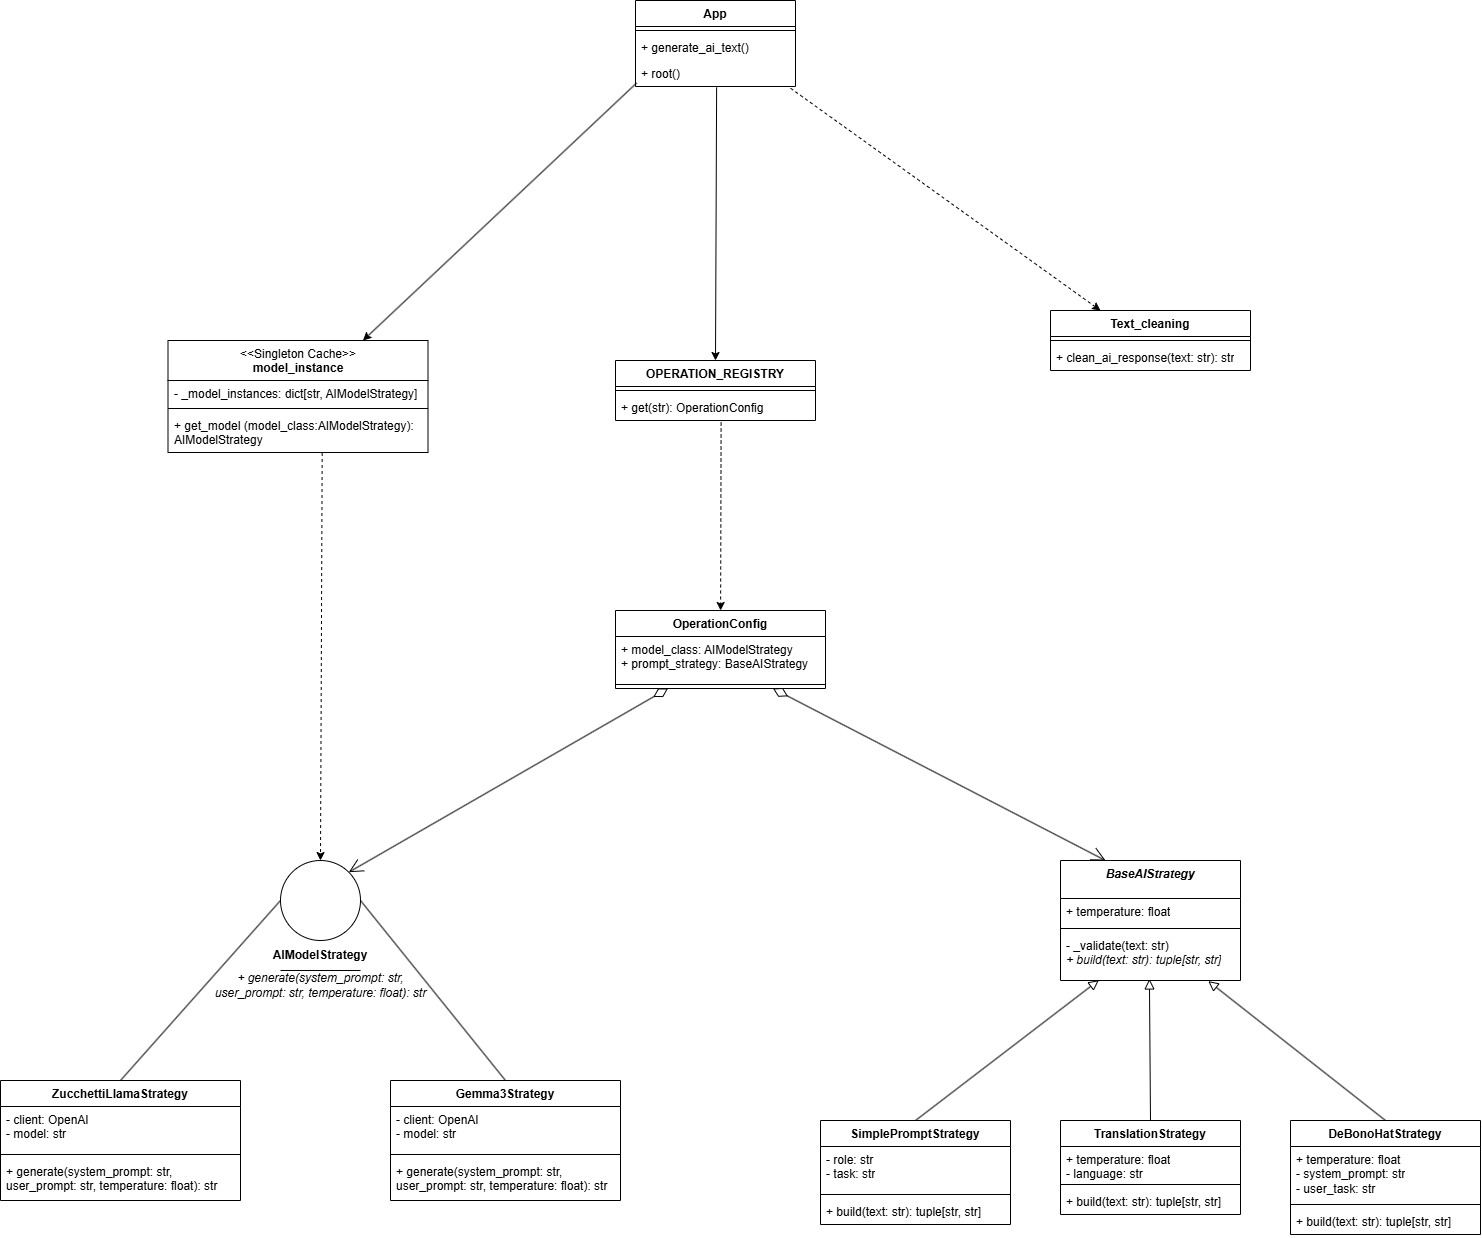
\includegraphics[width=1\textwidth]{../UMLimg/backend.jpg}
    \caption{Diagramma UML Backend: layered architecture e strategy pattern}
    \label{fig:uml_backend}
\end{figure}

\subsection{Strategy pattern}
Lo \textbf{Strategy} è un design pattern comportamentale il cui scopo principale è definire una famiglia di algoritmi, incapsularli in classi separate e renderli interscambiabili tra loro. Questo approccio permette agli algoritmi di variare in modo indipendente rispetto alle classi che li utilizzano, rendendo il codice modulare ed estensibile.

In pratica, questo pattern si rivela fondamentale quando esistono diverse varianti di una stessa operazione logica e si vuole permettere al sistema di cambiare comportamento a \textit{runtime}, mantenendo inalterata la struttura generale dell'interfaccia.

\paragraph{Struttura}
Strutturalmente, il pattern si compone di tre elementi chiave:
\begin{itemize}
    \item \textbf{Strategy (interfaccia)}: Un contratto generico comune supportato da tutti gli algoritmi della famiglia.
    \item \textbf{ConcreteStrategy}: Le classi concrete che implementano l'interfaccia \textit{Strategy}, definendo i dettagli di uno specifico algoritmo.
    \item \textbf{Context}: L'elemento che necessita dell'algoritmo. Esso mantiene un riferimento all'interfaccia, ignorando i dettagli implementativi della \textit{ConcreteStrategy} con cui è configurato.
\end{itemize}

\paragraph{Problema}
L’architettura iniziale del backend presentava un'eccessiva complessità logica dovuta alla gestione di molteplici modelli LLM e diverse logiche di prompting. La presenza di numerosi blocchi condizionali (if/else o switch) all'interno dell'entry point (\texttt{app.py}) rendeva il codice rigido, difficile da scalare e violava il principio di singola responsabilità (Single Responsibility Principle).

\paragraph{Vantaggi}
L'adozione di questo pattern porta tre importanti vantaggi:
\begin{enumerate}
    \item \textbf{Eliminazione degli statement condizionali}: Previene la proliferazione di classi client complesse e di lunghi blocchi \texttt{if/else} o \texttt{switch} per la selezione del comportamento.
    \item \textbf{Alternativa all'ereditarietà}: Fornisce un approccio basato sulla composizione, più flessibile rispetto all'estensione diretta delle classi.
    \item \textbf{Adesione ai principi SOLID (Open-Closed)}: Permette di aggiungere nuovi algoritmi semplicemente creando una nuova \textit{ConcreteStrategy}, senza modificare il \textit{Context} preesistente.
\end{enumerate}

\subsubsection{Applicazione 1: \gls{prompt} strategies (ai\_strategies.py)}
Questa prima applicazione del pattern gestisce la trasformazione del testo grezzo fornito dall'utente in un input strutturato e ottimizzato per l'IA.

\paragraph{BaseAIStrategy}
Definisce il contratto astratto comune per tutte le strategie di generazione dei \gls{prompt}.
\begin{itemize}
    \item\textbf{Attributi:}
\begin{itemize}
    \item \texttt{temperature}: Definisce il livello di creatività dell'output. Dichiara un valore di default pari a 0.5, sovrascrivibile nelle classi figlie.
\end{itemize}
    \item \textbf{Metodi:}
\begin{itemize}
    \item \texttt{\_validate()}: Metodo concreto ereditabile che \gls{verifica} la solidità dell'input (es. assicura che il testo non sia \texttt{None}, sollevando un \texttt{TypeError} in caso contrario).
    \item \texttt{build(text: str, \gls{prompt}: str)}: Metodo astratto che impone a ogni sottoclasse di restituire una tupla contenente due stringhe: il \gls{System prompt} (il ruolo dell'IA) e lo \gls{User prompt} (il task specifico).
\end{itemize}
\end{itemize}

\paragraph{SimplePromptStrategy}
Utilizzata per le operazioni editoriali standard (riassunto, correzione grammaticale, riscrittura). Mantiene la \gls{temperatura} di default a 0.5 e costruisce \gls{prompt} diretti impostando istruzioni ferree per evitare preamboli discorsivi.
\begin{itemize}
    \item\textbf{Attributi:}
\begin{itemize}
    \item \texttt{role} (str): Definisce l'identità dell'assistente (es. "Sei un correttore di bozze").
    \item \texttt{task} (str): Definisce l'istruzione specifica da eseguire.
\end{itemize}
    \item\textbf{Metodi:}
\begin{itemize}
    \item \texttt{build(text: str, \gls{prompt}: str)}: Combina \texttt{role} e \texttt{task} con il testo in ingresso per formare la tupla richiesta.
\end{itemize}
\end{itemize}

\paragraph{TranslationStrategy} 
Sottoclasse concreta specializzata nella gestione delle attività di traduzione multilingua. Questa classe ottimizza il \gls{prompt} per garantire che l'LLM operi esclusivamente come traduttore professionale, mantenendo la fedeltà linguistica. La \gls{temperatura} viene sovrascritta a 0.3 per favorire la massima fedeltà al testo originale.
\begin{itemize}
    \item \textbf{Attributi:}
\begin{itemize}
    \item language(str): Stringa che definisce la lingua di destinazione (es. "inglese", "cinese mandarino"). Questo attributo viene utilizzato per parametrizzare dinamicamente la richiesta al modello.
\end{itemize}
\item \textbf{Metodi:}
\begin{itemize}
    \item build(text: str, \gls{prompt}: str): Implementa la logica di costruzione del \gls{prompt} impostando un \gls{System \gls{Prompt}} rigido che definisce il ruolo (traduttore professionista) e i vincoli di output (nessuna frase introduttiva). Lo \gls{User \gls{Prompt}} include l'istruzione di traduzione specifica verso la lingua memorizzata nell'attributo language.
\end{itemize}
\end{itemize}

\paragraph{DeBonoHatStrategy}
Sottoclasse concreta progettata per implementare il metodo dei "Sei Cappelli per Pensare" di Edward de Bono. Questa strategia guida l'LLM verso un'analisi laterale e strutturata, forzando il modello a osservare il testo da una singola prospettiva cognitiva alla volta (emotiva, logica, creativa, ecc.).
\begin{itemize}
    \item \textbf{Attributi:}
\begin{itemize}
    \item system\_prompt (str): Memorizza le istruzioni di sistema complete che definiscono il ruolo, il tono e i vincoli del cappello specifico.
    \item user\_task (str): Memorizza le direttive di formattazione e le domande specifiche a cui il modello deve rispondere analizzando il testo.
    \item temperature (float): Il livello di creatività assegnato a quello specifico cappello.
\end{itemize}

\item \textbf{Metodi:}
\begin{itemize}
    \item build(text: str, \gls{prompt}: str): Utilizza le f-string per iniettare i valori di hat\_name e focus all'interno dei \gls{prompt}.
\end{itemize}
\end{itemize}

\paragraph{DistantWritingStrategy}
Sottoclasse concreta dedicata alla funzionalità di generazione creativa di contenuti. A differenza delle altre strategie, gestisce la particolarità di ricevere un input testuale diretto dall'utente (\gls{prompt}) accompagnato da un testo di contesto opzionale. La \gls{temperatura} viene sovrascritta a 0.7 per favorire una maggiore creatività del modello.
\begin{itemize}
    \item \textbf{Attributi:}
    \begin{itemize}
        \item role (str): Definisce l'identità creativa dell'IA (es. "Sei uno scrittore creativo di livello mondiale")
    \end{itemize}
    
    \item \textbf{Metodi:}
    \begin{itemize}
        \item build(text: str, \gls{prompt}: str): Implementa la logica di costruzione unendo l'istruzione dell'utente (\gls{prompt}) e l'eventuale text fornito come contesto. Imposta inoltre un \gls{System \gls{Prompt}} rigoroso per evitare frasi introduttive.
    \end{itemize}
\end{itemize}


% DIAGRAMMA DELLE CLASSI
\begin{figure}[H]
    \centering
    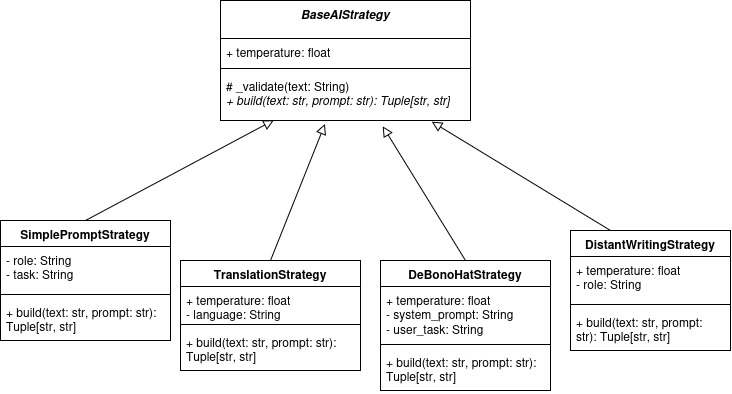
\includegraphics[width=0.8\textwidth]{../UMLimg/ai_strategies.jpg}
    \caption{Diagramma UMl: Strategy pattern applicato alle operazioni AI}
    \label{fig:uml_ai_strategy}
\end{figure}


\subsubsection{Applicazione 2: model strategies (model\_strategies.py)}
Questa seconda applicazione del pattern isola completamente i dettagli tecnici (\gls{Endpoint}, \gls{API} Keys, configurazione del client) necessari per comunicare con i diversi provider di Intelligenza Artificiale.

\paragraph{AIModelStrategy} 
Interfaccia comune per tutti i modelli linguistici IA.
\begin{itemize}
    \item \textbf{Metodi:}
\begin{itemize}
    \item \texttt{generate(self, system\_prompt, user\_prompt, temperature)}: Definisce il contratto per l'invocazione del modello, imponendo alle classi concrete di inviare i \gls{prompt} al fornitore e restituire la risposta come stringa pulita.
\end{itemize}
\end{itemize}

\paragraph{Implementazioni concrete (ZucchettiDeepSeekStrategy, Gemma3Strategy, Qwen3Strategy)}
Il sistema prevede tre implementazioni concrete che espongono in modo polimorfico i modelli \gls{Deepseek } (per operazioni di \gls{distant writing}),  \gls{Gemma 3} (per il pensiero laterale dei Sei Cappelli, riscrittura del testo e correzione grammaticale) e \gls{Qwen 3} (per operazioni di riassunto).
\begin{itemize}
    \item \textbf{Attributi:}
\begin{itemize}
    \item \texttt{client}: Istanza del client OpenAI-compatibile, inizializzata con \gls{API} key e base URL letti dalle variabili d'ambiente.
\end{itemize}
    \item \textbf{Metodi:}
\begin{itemize}
    \item \texttt{model} (str): Stringa identificativa del modello instradato (es. \texttt{"gemma3:4b"}).
    \item \texttt{generate(...)}: Implementa la logica di chiamata \gls{API}, inviando i messaggi nel formato richiesto dal protocollo \textit{ChatCompletion}. Estrae e restituisce esclusivamente il contenuto testuale, isolandolo dai metadati di rete (es. token consumati).
\end{itemize}
\end{itemize}

% DIAGRAMMA DELLE CLASSI
\begin{figure}[H]
    \centering
    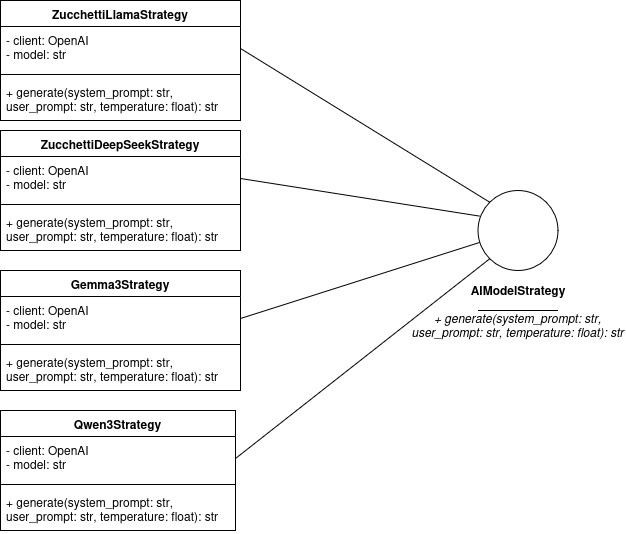
\includegraphics[width=0.8\textwidth]{../UMLimg/ai_model_strategies.jpg}
    \caption{Diagramma UMl: Strategy pattern applicato alla scelta dei LLM}
    \label{fig:uml_model_strategy}
\end{figure}


\subsubsection{Caching (get\_model)}
La funzione \texttt{get\_model(model\_class)} fornisce un’istanza unica per ciascun modello richiesto, evitando la creazione di più istanze della stessa classe e ottimizzando così l’utilizzo delle risorse.

Il meccanismo di caching è implementato tramite il decoratore \texttt{@lru\_cache} della libreria standard \texttt{functools}. Alla prima richiesta di un determinato modello, l’istanza viene creata e salvata; nelle chiamate successive con la stessa classe come argomento, \texttt{@lru\_cache} restituisce direttamente il riferimento già memorizzato.

L’utilizzo di \texttt{functools} consente di affidarsi a una soluzione robusta e consolidata, che gestisce in modo trasparente anche gli aspetti legati alla concorrenza tra thread, evitando la necessità di gestire dizionari globali o lock manuali all'interno del codice applicativo. Questo approccio riduce la complessità del codice e migliora l’affidabilità complessiva del sistema.

Nel contesto specifico dell’applicazione, la presenza di più istanze non avrebbe comportato criticità rilevanti, ma si è comunque scelto di adottare una soluzione più rigorosa per garantire maggiore solidità e aderenza alle buone pratiche di progettazione.



\newpage

% FRONTEND
\section{Frontend: architettura}
Il frontend del sistema è stato sviluppato utilizzando \textbf{\gls{React} 19}, adottando il pattern architetturale \textbf{MVVM} (Model-View-ViewModel). Questa scelta permette di separare nettamente la logica di business dalla logica di presentazione, facilitando il testing isolato dei componenti e la manutenibilità del codice.

L'organizzazione del progetto segue i principi della \textit{\gls{Feature-based Architecture}} (ispirata allo standard di settore \textbf{Bulletproof \gls{React}}). Invece di raggruppare i file per tipo (tutti i componenti insieme, tutti gli hook insieme), ogni funzionalità del sistema (es. \texttt{editor}, \texttt{history}) è isolata in un modulo autocontenuto che include i propri componenti, hook, store e definizioni di tipo.


% diagramma completo per MVVM
\begin{figure}[H]
    \centering
    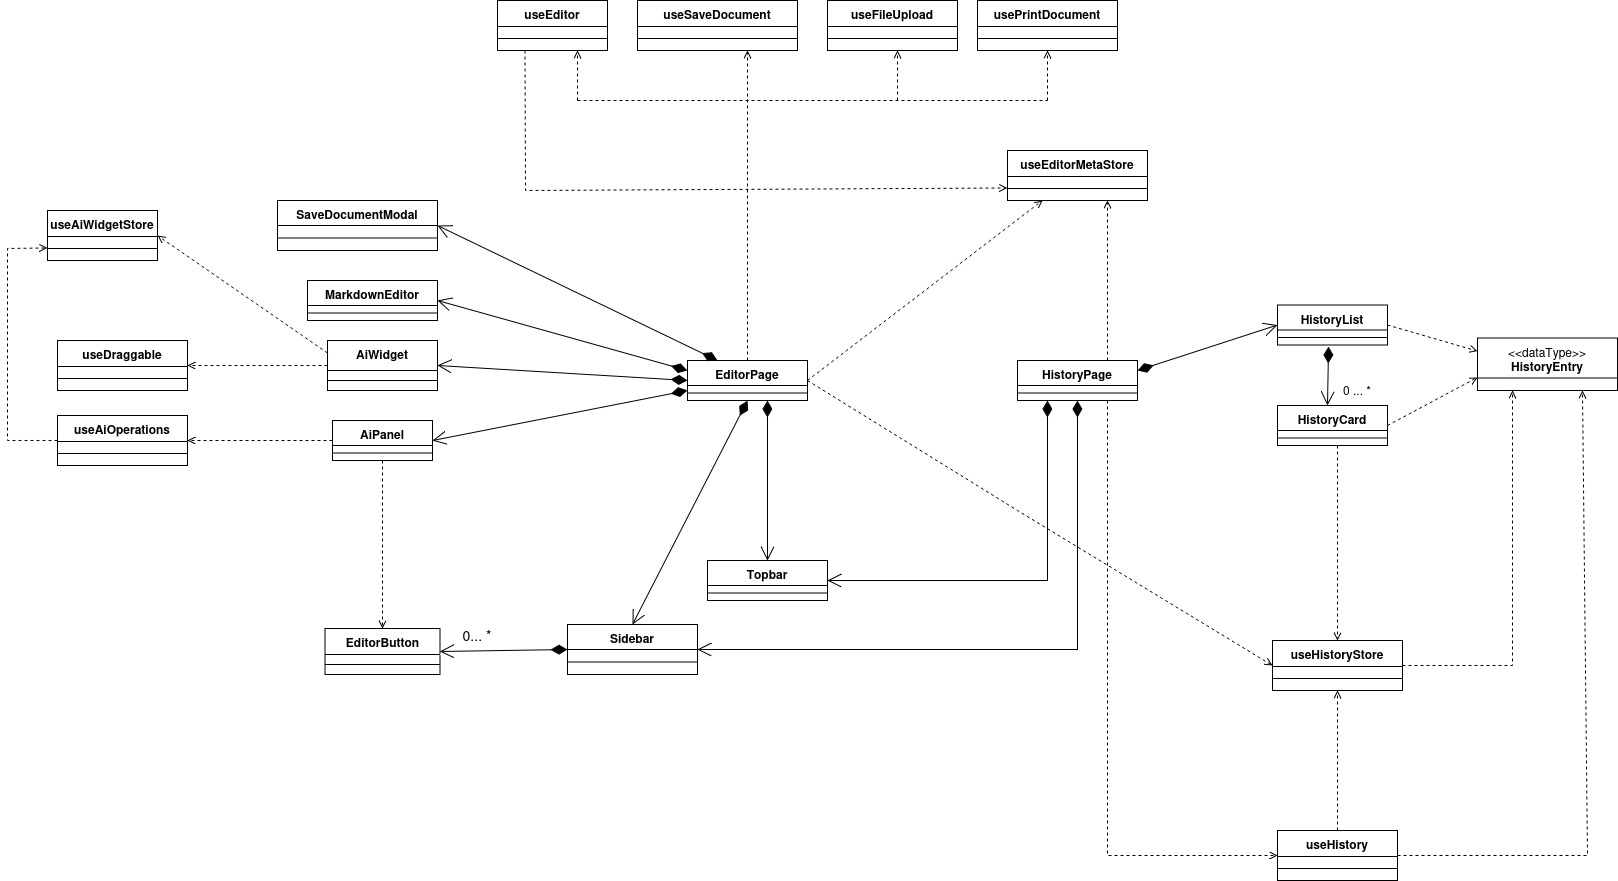
\includegraphics[width=1\textwidth]{../UMLimg/MVVM.jpg}
    \caption{Diagramma delle classi: architettura globale del frontend secondo il pattern MVVM.}
    \label{fig:uml_mvvm}
\end{figure}

\subsection{Model-View-ViewModel (MVVM)}
Il pattern architetturale \textbf{Model-View-ViewModel (MVVM)} è un'evoluzione dei pattern di presentazione (come MVC e MVP) progettata per separare rigorosamente lo sviluppo dell'interfaccia utente (UI) dalla logica di business e dallo stato dell'applicazione. È un pattern di riferimento per lo sviluppo client-side moderno e si adatta perfettamente al \gls{paradigma reattivo} di \gls{React}.

L'architettura si divide in tre strati le cui responsabilità sono nettamente separate:

\begin{itemize}
    \item \textbf{View (vista)}: Rappresenta l'interfaccia utente visibile (componenti \gls{JSX}/\gls{TSX}). Nel pattern MVVM, la View è prettamente dichiarativa e "passiva": non detiene la logica di business e non manipola direttamente i dati, ma si limita a renderizzare lo stato che le viene fornito e a delegare le azioni dell'utente ai livelli sottostanti.
    \item \textbf{ViewModel}: Funge da intermediario intelligente tra la View e il Model. È una rappresentazione dello stato e della logica adattata per una specifica vista. Nel nostro sistema è implementato tramite \textit{Custom Hooks}: mantiene lo stato UI temporaneo, espone i dati e i comandi eseguibili, cattura gli eventi generati dalla View (es. click, input) e orchestra le chiamate verso le \gls{API} o verso il Model.
    \item \textbf{Model (modello)}: Rappresenta il livello dei dati di dominio e della loro persistenza. Funge da \textit{Single Source of Truth} per l'applicazione. Non ha alcuna conoscenza della View; il suo compito è garantire la consistenza dei dati. Quando lo stato del Model cambia, i ViewModel ad esso sottoscritti (nel nostro caso tramite il pattern \textit{Observer} implementato da \gls{Zustand}) si aggiornano reattivamente, innescando di conseguenza un re-render della View associata.
\end{itemize}


% =======
% VIEW
% =======
\subsection{View: componenti di presentazione}
% DIAGRAMMA PER I COMPONENTI DELLA VIEW DELL'EDITOR
\begin{figure}[H]
    \centering
    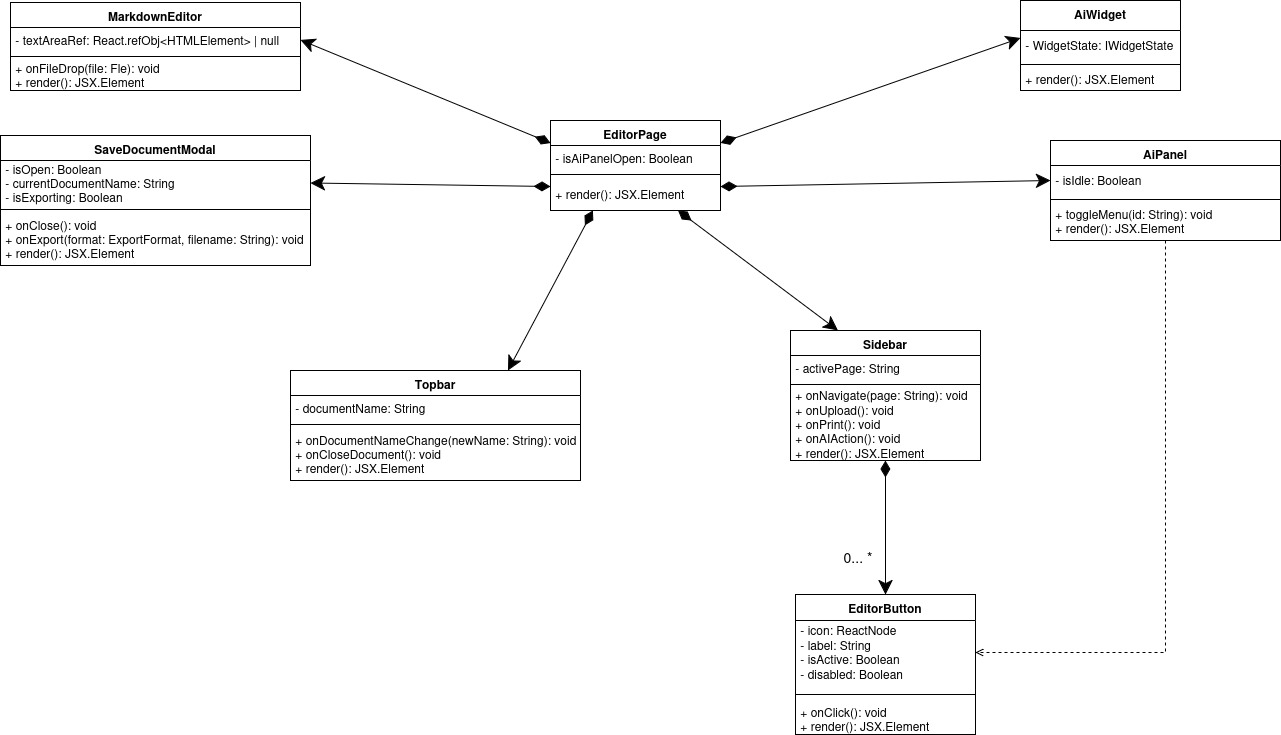
\includegraphics[width=1\textwidth]{../UMLimg/componenti_view_editor.jpg}
    \caption{Diagramma UML dei componenti della View: composizione di EditorPage}
    \label{fig:uml_view_editor}
\end{figure}

La View del sistema è realizzata tramite componenti \textbf{\gls{React} 19} di tipo funzionale. Per massimizzare la manutenibilità, il gruppo ha adottato un approccio basato su componenti \textit{presentational} (o "dumb"): non detengono logica di dominio, ma si limitano a riflettere lo stato ricevuto dal ViewModel e a propagare le interazioni dell'utente tramite callback. Questo isolamento garantisce che lo strato visivo sia agnostico rispetto alla business logic sottostante.

Di seguito sono descritti i componenti principali che compongono l'interfaccia.



% COMPONENTI
\subsubsection{Topbar}
% DESCRIZIONE
Barra superiore dell'applicazione posizionata in testa all'editor. Il suo scopo principale è visualizzare il nome del documento corrente tramite un campo di input editabile, permettendone la rinominazione rapida.

% PROPS (invece di attributi e metodi i componenti hanno dati e funzioni di callback nella props)
\paragraph{Props (Dati)}
\begin{itemize}
    \item \texttt{documentName: string} - nome attuale del documento in fase di editing.
\end{itemize}

\paragraph{Props (Callback)}
\begin{itemize}
    \item \texttt{onDocumentNameChange: (newName: string) => void} - funzione invocata alla modifica del titolo.
    \item \texttt{onCloseDocument: () => void} - funzione invocata per chiudere il documento corrente.
\end{itemize}


\subsubsection{Sidebar}
Barra laterale contenente i pulsanti di navigazione (switch tra editor e storico) e per le funzionalità operative (salvataggio, upload, stampa e azioni AI). Delega l'orchestrazione delle disabilitazioni (es. bloccare i bottoni AI quando si visualizza lo storico) tramite la logica della pagina padre.

\paragraph{Props (Dati)}
\begin{itemize}
    \item \texttt{activePage: 'editor' | 'history'} - determina la tipologia di view attualmente attiva per evidenziare il menu corretto (EditorPage o HistoryPage).
\end{itemize}

\paragraph{Props (Callback)}
\begin{itemize}
    \item \texttt{onNavigate: (page: 'editor' | 'history') => void} - aggiorna la view visualizzata.
    \item \texttt{onUpload: () => void} - innesca il caricamento di un file locale.
    \item \texttt{onSave: () => void} - innesca il flusso di salvataggio/esportazione.
    \item \texttt{onPrint: () => void} - invoca la stampa del documento.
    \item \texttt{onAiAction: () => void} - apre il pannello delle azioni di Intelligenza Artificiale.
\end{itemize}


\subsubsection{EditorButton}
Componente atomico e riutilizzabile che definisce l'interfaccia standard per tutti i bottoni della \texttt{Sidebar}. Gestisce i propri stati visivi (\texttt{isActive}, \texttt{disabled}) usando classi generate tramite \gls{CSS Modules}.

\paragraph{Props (Dati)}
\begin{itemize}
    \item \texttt{icon: ReactNode} - asset vettoriale/icona del bottone.
    \item \texttt{label: string} - etichetta testuale descrittiva.
    \item \texttt{isActive?: boolean} - determina lo stile di selezione.
    \item \texttt{disabled?: boolean} - inibisce l'interazione e applica lo stile di blocco.
\end{itemize}

\paragraph{Props (Callback)}
\begin{itemize}
    \item \texttt{onClick: () => void} - gestisce l'evento di pressione sul bottone.
\end{itemize}


\subsubsection{MarkdownEditor}
Componente delegato al rendering del corpo principale dell'area di scrittura. Consiste in un wrapper reattivo attorno a una \texttt{textarea} nativa su cui l'istanza di \gls{EasyMDE} viene "agganciata" dal ViewModel. Gestisce autonomamente gli eventi di trascinamento (\textit{drag-and-drop}) dei file esterni.

\paragraph{Props (Dati)}
\begin{itemize}
    \item \texttt{textAreaRef: \gls{React}.RefObject<HTMLTextAreaElement | null>} - puntatore fisico al nodo DOM su cui istanziare la libreria esterna.
\end{itemize}

\paragraph{Props (Callback)}
\begin{itemize}
    \item \texttt{onFileDrop?: (file: File) => void} - intercetta il rilascio di un file sull'area di testo.
\end{itemize}


\subsubsection{SaveDocumentModal}
Modale interattiva per la configurazione dell'esportazione del documento. Mantiene traccia dello stato locale (formato selezionato, modifiche al nome) e applica tecniche di \textit{sanitizzazione} sul testo immesso prima di confermare.

\paragraph{Props (Dati)}
\begin{itemize}
    \item \texttt{isOpen: boolean} - controlla la visibilità a schermo.
    \item \texttt{currentDocumentName: string} - funge da valore predefinito e \textit{placeholder} nell'input text.
    \item \texttt{isExporting?: boolean} - stato transitorio che disabilita i controlli durante l'elaborazione del download.
\end{itemize}

\paragraph{Props (Callback)}
\begin{itemize}
    \item \texttt{onClose: () => void} - innesca la chiusura senza salvataggio.
    \item \texttt{onExport: (format: ExportFormat, filename: string) => void} - passa i parametri sanitizzati al ViewModel per l'esecuzione del salvataggio.
\end{itemize}

\subsubsection{AiPanel}
Componente laterale di controllo dedicato alla selezione e all'invocazione delle operazioni di Intelligenza Artificiale. Funge da interfaccia di comando strutturata, organizzando le funzionalità in categorie logiche (operazioni testuali, strumenti di analisi De Bono, traduzioni multilingua).

\paragraph{Responsabilità e logica}
Essendo un componente connesso, l'\texttt{AiPanel} non riceve \textit{props} esterne, ma incapsula le seguenti logiche:
\begin{itemize}
    \item \textbf{Orchestrazione comandi}: Mappa la pressione dei bottoni (\texttt{EditorButton}) verso le funzioni esposte dal ViewModel \texttt{useAiOperations}.
    \item \textbf{Gestione menù annidati}: Gestisce localmente lo stato di apertura/chiusura dei sottomenù (es. la lista delle lingue per la traduzione) tramite un set di identificatori (\texttt{openMenus}).
    \item \textbf{Controllo di flusso}: Interroga lo store \texttt{useAiWidgetStore} per verificare se il sistema è in stato di attesa (\texttt{isIdle}); in caso di generazione già in corso, disabilita globalmente i propri comandi per prevenire richieste concorrenti.
\end{itemize}


\subsubsection{AiWidget}
Componente flottante e interattivo delegato alla gestione visuale del ciclo di vita di una richiesta AI. Il widget si sovrappone all'interfaccia principale e guida l'utente attraverso le diverse fasi dell'operazione: dall'input di parametri aggiuntivi (\gls{prompt} personalizzati) fino alla visualizzazione e all'inserimento del risultato nell'editor.

\paragraph{Caratteristiche principali}
Il componente si distingue per un'alta dinamicità e flessibilità architetturale:
\begin{itemize}
    \item \textbf{Rendering polimorfico}: Non possiede un markup statico unico. Utilizza degli stati per delegare il rendering del proprio corpo (\texttt{body}) e delle azioni (\texttt{actions}) all'oggetto di stato attualmente attivo nello store (\texttt{widgetState}).
    \item \textbf{Esperienza utente}: Grazie all'hook \texttt{useDraggable}, il widget può essere spostato liberamente dall'utente all'interno dell'area di lavoro (tramite \textit{drag-and-drop} sull'header), evitando di coprire porzioni di testo rilevanti durante la consultazione dei risultati.
    \item \textbf{Disaccoppiamento}: È totalmente agnostico rispetto all'operazione specifica che lo ha attivato; si limita a riflettere lo stato della "macchina a stati" sottostante definita nel ViewModel.
\end{itemize}


% DIAGRAMMA PER I COMPONENTI DELLA VIEW DELLO STORICO
\begin{figure}[H]
    \centering
    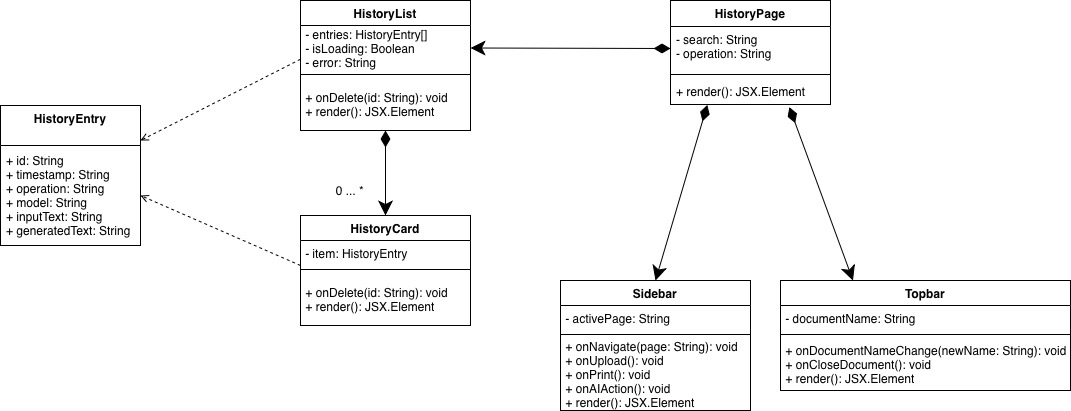
\includegraphics[width=1\textwidth]{../UMLimg/componenti_view_storico.jpg}
    \caption{Diagramma UML dei componenti della View: composizione di HistoryPage}
    \label{fig:uml_view_storico}
\end{figure}

\subsubsection{HistoryList}
Componente per il rendering aggregato dello storico delle generazioni degli LLM. Gestisce internamente l'alternanza visiva tra stati di transizione (caricamento, errore) e lo stato di successo, delegando la visualizzazione del singolo nodo a \texttt{HistoryCard}.

\paragraph{Props (Dati)}
\begin{itemize}
    \item \texttt{items: HistoryItem[]} - array di oggetti rappresentanti le generazioni AI.
    \item \texttt{isLoading: boolean} - abilita il rendering dell'indicatore di caricamento.
    \item \texttt{error: string | null} - stringa che riporta un messaggio d'errore nel caricamento della cronologia (se presente).
\end{itemize}

\paragraph{Props (Callback)}
\begin{itemize}
    \item \texttt{onDelete: (id: string) => void} - propaga verso l'alto la richiesta di rimozione di uno specifico elemento.
\end{itemize}


\subsubsection{HistoryCard}
Componente granulare che rappresenta la singola scheda di interazione AI. Incapsula logiche puramente visive tramite \texttt{useState}, quali l'espansione/compressione di testi lunghi e il feedback del pulsante di copia negli appunti.

\paragraph{Props (Dati)}
\begin{itemize}
    \item \texttt{item: HistoryItem} - struttura dati completa dell'interazione (\gls{prompt}, output, modello usato, data).
\end{itemize}

\paragraph{Props (Callback)}
\begin{itemize}
    \item \texttt{onDelete: (id: string) => void} - gestisce l'eliminazione di una card specifica.
\end{itemize}


\newpage
% ============
% VIEW-MODEL
% ============
\subsection{ViewModel: custom hooks e logica di business}
% GRAFICO per gli hooks dell'editor
\begin{figure}[H]
    \centering
    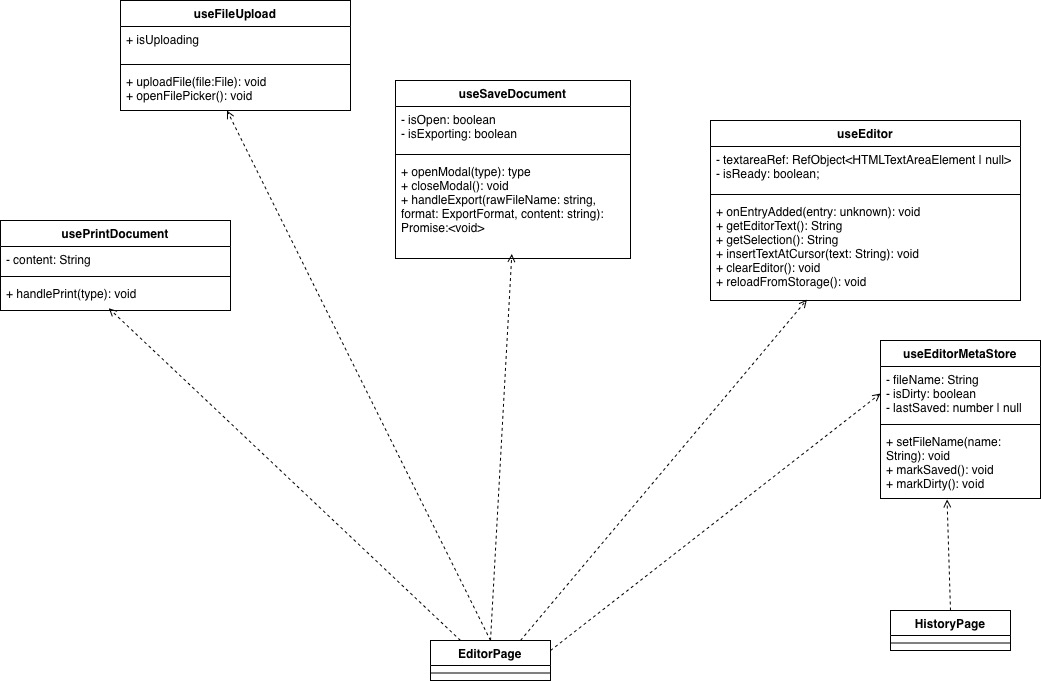
\includegraphics[width=1\textwidth]{../UMLimg/hooks_editor.jpg}
    \caption{UML hooks editor}
    \label{fig:uml_hooks_Editor}
\end{figure}

Il ViewModel funge da intermediario tra il Model e la View ed è implementato tramite \textbf{Custom Hooks} specializzati. Ogni hook rispetta il \textit{Single Responsibility Principle} (SRP).
Il ViewModel ha la responsabilità di:
\begin{itemize}
    \item Esporre i dati e lo stato degli store alle View in un formato pronto per la visualizzazione.
    \item Gestire la logica di interazione complessa (ad esempio, l'orchestrazione delle \gls{API} AI tramite la Facade \texttt{aiCall}).
    \item Manipolare direttamente le istanze di librerie esterne, come \textbf{\gls{EasyMDE}} per l'editor \gls{Markdown}, isolandone la complessità tecnica all'interno di hook dedicati.
\end{itemize}

\subsubsection{useEditor}
Hook centrale dell'applicazione. Gestisce il ciclo di vita dell'istanza \gls{EasyMDE} (creazione al mount, distruzione al cleanup). Implementa l'auto-save con tecnica di \textit{debounce} (500 ms) per evitare scritture eccessive su disco. Fornisce all'esterno un'interfaccia solida per interagire con il testo.

\paragraph{Stato/Valori di ritorno}
\begin{itemize}
    \item \texttt{textAreaRef: \gls{React}.RefObject<HTMLTextAreaElement | null>} - riferimento iniettato nella view.
    \item \texttt{isReady: boolean} - \textit{flag} che indica la completa inizializzazione del motore di rendering \gls{Markdown}.
\end{itemize}

\paragraph{Funzioni esposte}
\begin{itemize}
    \item \texttt{getEditorText: () => string} - restituisce l'intero contenuto testuale corrente.
    \item \texttt{getSelection: () => string} - estrae la porzione di testo evidenziata dall'utente.
    \item \texttt{insertTextAtCursor: (text: string) => void} - inietta testo elaborato (es. output AI) nella posizione attuale del cursore.
    \item \texttt{clearEditor: () => void} - resetta l'area di lavoro.
    \item \texttt{reloadFromStorage: () => void} - forza la sincronizzazione con il LocalStorage.
\end{itemize}

\subsubsection{useSaveDocument}
Coordina il flusso di esportazione asincrono. Orchestra in sequenza la composizione sicura del filename, il download fisico (mediato dal file \texttt{fileHandler.ts}) e il dispatch verso lo store per aggiornare il timestamp di salvataggio. In caso di errore fallisce silenziosamente mantenendo la modale aperta per un nuovo tentativo.

\paragraph{Stato/Valori di ritorno}
\begin{itemize}
    \item \texttt{isOpen: boolean} - stato di visibilità della modale di salvataggio.
    \item \texttt{isExporting: boolean} - stato transitorio che indica se il processo di download è in corso.
\end{itemize}

\paragraph{Funzioni esposte}
\begin{itemize}
    \item \texttt{openModal: () => void} - innesca l'apertura della modale.
    \item \texttt{closeModal: () => void} - innesca la chiusura della modale.
    \item \texttt{handleExport: (rawFilename: string, format: ExportFormat, content: string) => Promise<void>} - processa la richiesta di esportazione, applica la mappa dei MIME type ed esegue il download.
\end{itemize}

\subsubsection{useFileUpload}
Gestisce il caricamento asincrono tramite \texttt{FileReader}. Esegue controlli preventivi (\gls{validazione} del formato supportato \texttt{.md} o \texttt{.txt}, dimensione massima 5 MB) e previene la perdita accidentale di dati non salvati bloccando l'utente e chiedendogli conferma tramite \texttt{window.confirm}.

\paragraph{Stato/Valori di ritorno}
\begin{itemize}
    \item \texttt{fileInputRef: \gls{React}.RefObject<HTMLInputElement>} - riferimento fisico all'input nascosto di tipo \texttt{file} nel DOM.
\end{itemize}

\paragraph{Funzioni esposte}
\begin{itemize}
    \item \texttt{triggerFileInput: () => void} - simula il click sull'input nascosto per aprire la finestra di dialogo di sistema.
    \item \texttt{handleFileUpload: (event: \gls{React}.ChangeEvent<HTMLInputElement>) => Promise<void>} - intercetta il file selezionato, lo valida e ne legge il contenuto testuale.
\end{itemize}

\subsubsection{usePrintDocument}
Isola e rende testabile la logica di invocazione della stampa di sistema (\texttt{window.print()}). Implementa \textit{guard clauses} per impedire l'avvio del processo se il documento risulta vuoto.
Questo hook opera esclusivamente in modo imperativo, non ha quindi nessuno stato locale esposto.

\paragraph{Funzioni esposte}
\begin{itemize}
    \item \texttt{handlePrint: (content: string) => void} - \gls{verifica} la lunghezza del contenuto e innesca la stampa del browser o genera un errore visivo.
\end{itemize}


\subsubsection{useHistory}
% diagramma che mostra i collegamenti tra view storico e hooks + store
\begin{figure}[H]
    \centering
    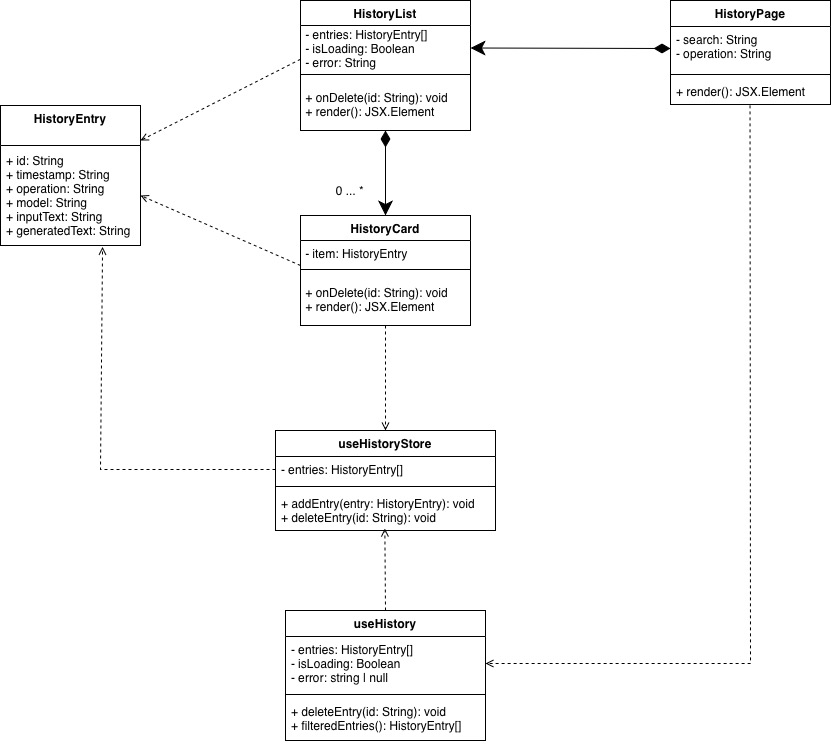
\includegraphics[width=1\textwidth]{../UMLimg/hooks_storico.jpg}
    \caption{Architettura del modulo History: interazione tra l'hook useHistory e lo store \gls{Zustand}.}
    \label{fig:uml_hooks_storico}
\end{figure}


Interfaccia la View con lo store dedicato (\texttt{useHistoryStore}), estraendo le interazioni passate. Per garantire alte prestazioni e fluidità UI, tramite \texttt{useMemo} applica dinamicamente i filtri di ricerca e l'ordinamento cronologico, assicurando che lo strato di presentazione riceva sempre informazioni formattate senza subire calcoli ridondanti.



\paragraph{Stato/Valori di ritorno}
\begin{itemize}
    \item \texttt{entries: HistoryEntry[]} - array delle interazioni, eventualmente filtrato e ordinato in base ai criteri correnti.
    \item \texttt{isLoading: boolean} - indica se i dati sono ancora in fase di recupero dal LocalStorage o dallo store.
    \item \texttt{error: string | null} - eventuale stringa di errore occorso durante il fetching della history.
\end{itemize}

\paragraph{Funzioni esposte}
\begin{itemize}
    \item \texttt{deleteEntry: (id: string) => void} - innesca la cancellazione di una specifica riga dallo storico persistente.
\end{itemize}


\subsubsection{useAiOperations}
% grafico con il dettaglio di useAiOperaions e useDraggable
\begin{figure}[H]
    \centering
    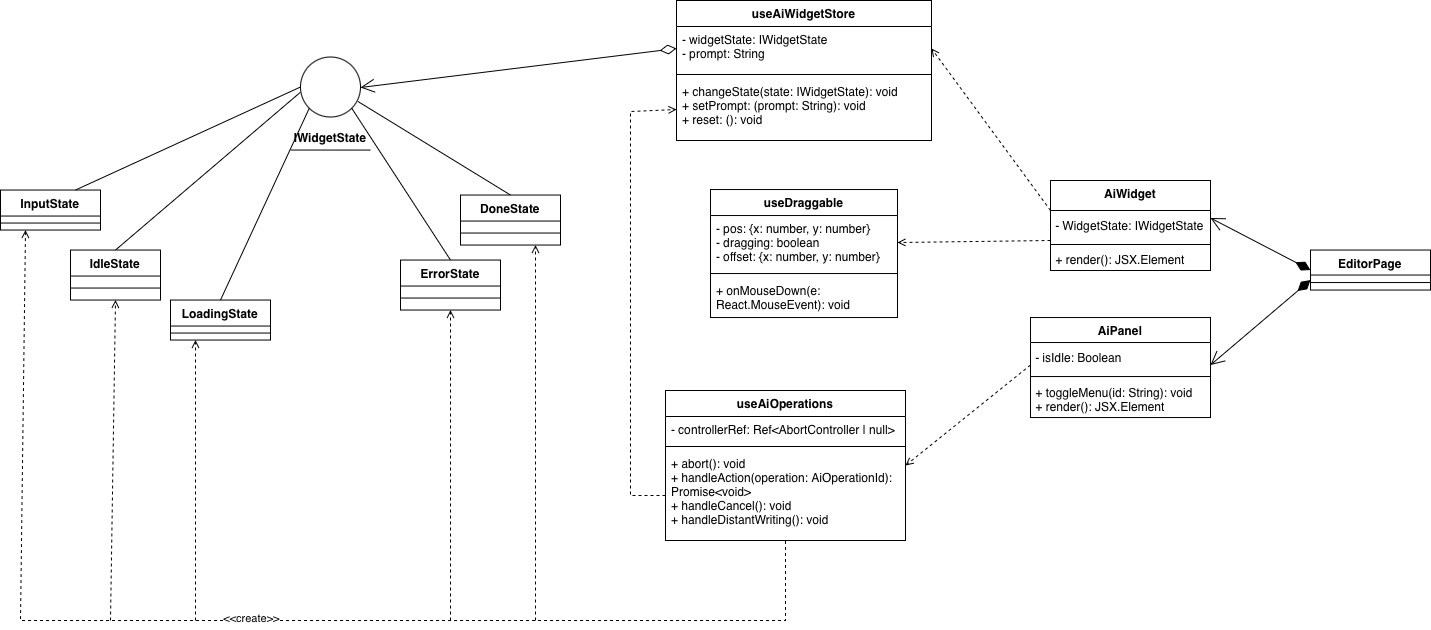
\includegraphics[width=1\textwidth]{../UMLimg/hooks_ai.jpg}
    \caption{UML funzionalità AI: interazione tra ViewModel, Store globale e stati del widget.}
    \label{fig:uml_hooks_ai}
\end{figure}
Hook \gls{orchestratore} dedicato alla gestione delle interazioni con l'Intelligenza Artificiale. Funge da regista tra la View, i servizi di rete e lo stato globale del widget, isolando la logica di invocazione della Facade \texttt{aiCall} e gestendo il ciclo di vita delle richieste asincrone tramite un \texttt{AbortController} mantenuto in un \texttt{\gls{React}.RefObject} (\texttt{controllerRef}). È l'unico punto del sistema responsabile della creazione delle istanze delle classi di stato, nelle quali inietta le callback operative necessarie, e dell'invocazione di \texttt{changeState} sullo store \texttt{aiWidgetStore}.

\paragraph{Props (dipendenze)}
L'hook riceve in ingresso un oggetto di configurazione per interagire con l'editor in modo disaccoppiato:
\begin{itemize}
    \item \texttt{getEditorText: () => string} - funzione per recuperare il contenuto totale.
    \item \texttt{getSelection: () => string} - funzione per recuperare il testo selezionato.
    \item \texttt{insertText: (text: string) => void} - funzione per iniettare il risultato nell'editor.
    \item \texttt{onEntryAdded?: (entry: any) => void} - callback opzionale per il salvataggio nello storico.
\end{itemize}

\paragraph{Gestione dell'annullamento}
Prima di ogni nuova richiesta, l'hook invoca \texttt{abort()} sull'eventuale controller precedente per annullare operazioni in corso, creando poi un nuovo \texttt{AbortController}. La funzione interna \texttt{handleCancel} incapsula questo comportamento e lo espone agli stati che ne necessitano (es. \texttt{LoadingState}).

\paragraph{Funzioni esposte}
\begin{itemize}
    \item \texttt{handleAction: (operation: AiOperationId) => Promise<void>} - funzione principale che avvia il flusso AI. Intercetta il caso \texttt{"distant\_writing"} e lo delega a \\ \texttt{handleDistantWriting}; per tutte le altre operazioni, esegue direttamente il flusso standard.
    \item \texttt{handleDistantWriting: () => void} - funzione che inizializza il flusso con input utente, portando il widget in \texttt{InputState} con la callback \texttt{onConfirm} preconfigurata.
\end{itemize}

\subsubsection{useDraggable}
Hook di utilità incaricato di gestire la logica di posizionamento e trascinamento (\textit{drag-and-drop}) di componenti flottanti all'interno dell'interfaccia. Astrae la gestione dei \textit{listener} degli eventi del mouse (\texttt{mousemove}, \texttt{mouseup}) registrati a livello di \texttt{window}, garantendo che il trascinamento funzioni correttamente anche quando il cursore fuoriesce dai limiti del componente durante il movimento rapido.

\paragraph{Scelte implementative}
L'hook adotta \texttt{useRef} per i campi \texttt{dragging} e \texttt{offset}, anziché \texttt{useState}: essendo questi valori aggiornati ad alta frequenza durante il \textit{drag}, evitare re-render inutili è fondamentale per la fluidità visiva. Solo \texttt{pos} è dichiarato con \texttt{useState}, poiché è il dato che deve propagarsi al componente per aggiornarne il rendering. Il \textit{listener} \texttt{onMouseDown} è stabilizzato tramite \texttt{useCallback}, evitando che il riferimento alla funzione cambi ad ogni \textit{render} del componente ospitante. Al rilascio del mouse (\texttt{mouseup}), i \textit{listener} vengono rimossi tramite \texttt{removeEventListener}, prevenendo accumuli di \textit{handler} e potenziali \textit{memory leak}.

\paragraph{Stato/Valori di ritorno}
\begin{itemize}
    \item \texttt{pos: \{ x: number, y: number \}} - coordinate spaziali attuali del componente, aggiornate reattivamente durante il trascinamento.
\end{itemize}

\paragraph{Funzioni esposte}
\begin{itemize}
    \item \texttt{onMouseDown: (e: \gls{React}.MouseEvent) => void} - \textit{handler} da collegare all'area sensibile al trascinamento (es. l'header di \texttt{AiWidget}). Al momento del click calcola l'offset tra la posizione del cursore e l'origine del componente, poi registra i \textit{listener} a livello di \texttt{window} per tracciare il movimento e rilevare il rilascio.
\end{itemize}


\newpage
% =======
% MODEL
% =======
\subsection{Model: stato e persistenza}
\begin{figure}[H]
    \centering
    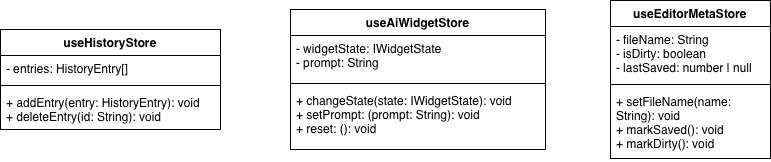
\includegraphics[width=1\textwidth]{../UMLimg/model.jpg}
    \caption{model}
    \label{fig:model}
\end{figure}
Il Model rappresenta lo strato dei dati e della loro persistenza. Nel sistema non è una struttura passiva, ma è implementato tramite store globali gestiti con \textbf{\gls{Zustand}}, che fungono da unica fonte di verità (\textit{Single Source of Truth}) per lo stato dell'applicazione.
Sono presenti tre store principali:
\begin{itemize}
    \item \texttt{useEditorMetaStore}: Gestisce i metadati dell'editor attivo, ovvero il nome del file (\texttt{fileName}), lo stato di modifica non salvata (\texttt{isDirty}) e il timestamp dell'ultimo salvataggio (\texttt{lastSaved}). Tramite il middleware \texttt{persist} di \gls{Zustand}, sincronizza automaticamente questo stato nel \texttt{localStorage} del browser, garantendo che i dati sopravvivano al riavvio della pagina.
    \item \texttt{useHistoryStore}: Gestisce l'elenco delle generazioni AI prodotte. Ogni voce è modellata dall'interfaccia \texttt{HistoryEntry}. Anche questo store utilizza il \texttt{localStorage} per rendere lo storico persistente tra le sessioni.
    \item \texttt{aiWidgetStore}: Gestisce lo stato transitorio e non persistente dell'interfaccia dedicata all'intelligenza artificiale. A differenza degli altri store del sistema, questo modulo non utilizza il middleware di persistenza, garantendo che il widget ritorni sempre alla condizione iniziale di riposo (\texttt{IdleState}) ad ogni ricaricamento della pagina. Al suo interno memorizza l'istanza dell'oggetto di stato corrente (\texttt{widgetState}), permettendo il rendering polimorfo del widget, e mantiene il testo temporaneo inserito dall'utente per le richieste personalizzate (\texttt{\gls{prompt}}).
\end{itemize}

\textit{Nota}: Il contenuto testuale effettivo dell'editor, per ragioni di performance legate alla natura della libreria \gls{EasyMDE}, non transita attraverso lo store globale, ma viene salvato e sincronizzato direttamente in una chiave dedicata del \texttt{localStorage} gestita dal ViewModel dell'editor.


\newpage

% DEPENDENCY INJECTION e PAGINE
\subsection{Orchestrazione e Dependency Injection}
A legare i tre strati architetturali (Model, View, ViewModel) intervengono le \textbf{Page} (\texttt{EditorPage} e \texttt{HistoryPage}). Questi componenti non appartengono né alla View pura (poiché conoscono lo stato globale e gli hook) né al ViewModel (poiché restituiscono markup \gls{JSX}). Essi fungono da \textbf{Orchestratori}.

Il ruolo dell'\gls{orchestratore} è quello di istanziare i ViewModel, leggere lo stato dai Model e far fluire i dati e le callback verso il basso (tramite \textit{\gls{prop drilling}} limitato a un solo livello) per distribuirli alle View.

\subsubsection{EditorPage: \gls{orchestratore} dell'editor}
\texttt{EditorPage} rappresenta l'entry point principale dell'applicazione e coordina la logica complessa dell'editor. Si occupa di:
\begin{itemize}
    \item \textbf{Gestione dello stato locale}: Controlla stati puramente visivi e non condivisi, come l'apertura/chiusura del pannello AI (\texttt{isAiPanelOpen}).
    \item \textbf{Collegamento al Model}: Legge e aggiorna i metadati del documento (es. \texttt{fileName}, \texttt{isDirty}) richiamando \texttt{useEditorMetaStore}.
    \item \textbf{Istanziazione del ViewModel}: Monta gli hook dedicati (\texttt{useEditor}, \texttt{useSaveDocument}, \texttt{useFileUpload}, \texttt{usePrintDocument}).
    \item \textbf{Composizione degli handler}: Crea funzioni ponte tra la View e il ViewModel. Ad esempio, \texttt{handleExportWithContent} recupera prima il testo tramite \texttt{editor.getEditorText()} e lo passa al ViewModel di salvataggio; \texttt{handleCloseDocument} \gls{verifica} la presenza di modifiche non salvate tramite \texttt{window.confirm} prima di resettare l'editor.
\end{itemize}

\subsubsection{HistoryPage: \gls{orchestratore} dello storico}
\texttt{HistoryPage} coordina la vista della cronologia delle generazioni AI. Rispetto all'editor, ha un ruolo più limitato:
\begin{itemize}
    \item \textbf{Stato dei filtri}: Mantiene localmente i criteri di ricerca dell'utente (\texttt{search} per il testo, \texttt{operation} per il tipo di task AI).
    \item \textbf{Delega la logica}: Passa i filtri dinamici al ViewModel \texttt{useHistory}, che si occupa del ricalcolo e dell'ordinamento delle voci.
    \item \textbf{Riutilizzo della UI}: Importa la \texttt{Topbar} in modalità sola lettura (passando \texttt{() => \{\}} come callback di modifica) e la \texttt{Sidebar}, garantendo coerenza visiva con l'editor pur disabilitando i comandi non pertinenti.
\end{itemize}


\subsubsection{Dependency Injection (DI)}
La \textbf{Dependency Injection} è un pattern architetturale fondamentale dell'Ingegneria del Software, volto a implementare il principio dell'Inversione del Controllo (IoC). Consiste nel fornire a un oggetto o a una funzione le dipendenze di cui ha bisogno dall'esterno, anziché permettere che sia il componente stesso a istanziarle o importarle in modo rigido. Questo approccio riduce l'accoppiamento (\textit{tight coupling}) tra i moduli, aumenta la coesione e rende il sistema altamente modulare e testabile.

\paragraph{Applicazione nel frontend}
Nel sistema \textit{Second Brain}, questo principio è stato adottato in modo trasversale nell'orchestrazione dei ViewModel. Per evitare dipendenze circolari o un accoppiamento rigido tra domini funzionali diversi, i \textit{custom hook} non importano mai la logica di altri hooks.

Il caso più evidente si trova nell'istanza di \texttt{useEditor}: questo hook non importa lo store \texttt{useHistoryStore} per salvare le generazioni e ignora del tutto l'esistenza dello storico. Al contrario, è l'\gls{orchestratore} (\texttt{EditorPage}) che si fa carico di prelevare l'azione \texttt{addEntry} dallo store dello storico per poi iniettarla all'interno di \texttt{useEditor} tramite la callback \texttt{onEntryAdded}.

Questo approccio garantisce che ogni hook sia modulare e testabile in totale isolamento fornendo dei semplici \textit{mock} al momento dei test.


\newpage

\section{Frontend: design pattern}
La progettazione del frontend di \textit{Second Brain} ha fatto uso di design pattern strutturali 
orientati alla semplificazione dell'interfaccia tra i moduli e al disaccoppiamento tra la logica 
di presentazione e i dettagli implementativi della comunicazione di rete. Nel sistema, la 
comunicazione con il backend non avviene mai tramite chiamate dirette alla libreria esterna 
\texttt{Axios}: è stata invece adottata un'architettura a due pattern distinti e complementari, 
in cui il Facade si occupa del \textit{come} comunicare con il server, e il Gateway del 
\textit{cosa} richiedere, garantendo che View e ViewModel rimangano agnostici rispetto a 
entrambi gli aspetti.

\subsection{Facade pattern - apiClient.ts}
Il pattern \textbf{Facade} è un design pattern strutturale il cui scopo principale è fornire un'interfaccia unica e semplificata per gestire un sottosistema complesso. L'obiettivo è nascondere le dipendenze e i dettagli implementativi al client, fornendogli un singolo punto di accesso di alto livello. Questo comporta tre vantaggi architetturali principali: riduce la superficie di contatto tra il client e il sottosistema (\textit{loose coupling}); diminuisce la complessità generale favorendo l'organizzazione in layer netti; facilita la scrittura di test automatici tramite \textit{mocking} e riduce l'impatto di eventuali refactoring.

\subsubsection{Problema}
Senza un punto di accesso centralizzato, ogni componente o ViewModel che necessita di comunicare con il backend dovrebbe configurare autonomamente la libreria Axios, gestire i propri errori di rete e implementare la logica di cancellazione delle richieste. Questo approccio porterebbe a duplicazione del codice, comportamenti eterogenei in caso di errore e un forte accoppiamento tra la logica di presentazione e i dettagli implementativi del trasporto HTTP.

\subsubsection{Applicazione}
Il file \texttt{apiClient.ts} funge da Facade per il sottosistema di networking. Il suo scopo è nascondere la complessità di Axios e fornire un'interfaccia semplificata e centralizzata per tutta l'applicazione. Invece di configurare i parametri di rete in ogni componente, il Facade si occupa di:
\begin{itemize}
\item \textbf{Centralizzazione della configurazione}: gestisce in un unico punto la \texttt{baseURL}, il timeout e gli header standard, leggendone i valori dalle variabili d'ambiente (\texttt{\gls{VITE}\_API\_BASE\_URL}, \texttt{\gls{VITE}\_API\_TIMEOUT}) con fallback ai valori di default. Qualsiasi modifica ai parametri di connessione richiede interventi esclusivamente in questo file.
\item \textbf{Normalizzazione degli errori}: tramite un response interceptor, intercetta qualsiasi fallimento (assenza di connessione, errori HTTP 4xx/5xx, timeout, richieste annullate tramite \texttt{AbortSignal}) e lo trasforma in un oggetto \texttt{Error} standard attraverso la funzione pura \texttt{transformApiError}. Questo garantisce che il resto dell'applicazione riceva sempre errori omogenei, indipendentemente dalla causa tecnica del problema.
\item \textbf{Gestione unificata della cancellazione}: integra il supporto nativo all'\texttt{AbortSignal}, permettendo ai ViewModel di interrompere richieste pendenti (ad esempio quando l'utente annulla un'operazione AI in corso) senza che questa logica debba essere replicata nei singoli componenti.
\end{itemize}

\subsection{Gateway - aiCall.ts}
Mentre il Facade gestisce il \textit{come} comunicare, \texttt{aiCall.ts} agisce come un Gateway applicativo. Questo pattern ha il compito di incapsulare l'accesso a una risorsa esterna specifica — in questo caso, le funzionalità di Intelligenza Artificiale del backend — esponendo un'interfaccia orientata al dominio anziché al protocollo HTTP.

\subsubsection{Problema}
Senza un Gateway, ogni ViewModel che necessita di invocare un'operazione AI dovrebbe conoscere l'URL esatto dell'\gls{endpoint}, costruire manualmente il payload JSON nel formato atteso dal backend e estrarre il testo generato dalla struttura della risposta HTTP. Questo comporterebbe una dipendenza diretta tra la logica di presentazione e i dettagli implementativi del servizio AI: qualsiasi modifica all'\gls{endpoint} o al formato dei dati richiederebbe interventi su tutti i componenti che effettuano la chiamata.

\subsubsection{Applicazione}
Il Gateway astrae l'\gls{endpoint} specifico (\texttt{/ai/generate}) e traduce il linguaggio del frontend in quello richiesto dal server:
\begin{itemize}
\item \textbf{Interfaccia di dominio}: espone il metodo \texttt{executeOperation}, che accetta parametri tipizzati (\texttt{AiRequestPayload}, \texttt{AbortSignal}) e restituisce direttamente una \texttt{Promise<string>}, nascondendo la struttura raw della risposta HTTP (\texttt{AiResponse.generated\_text}) ai livelli superiori.
\item \textbf{Contratto dei tipi}: il tipo enumerato \texttt{AiOperationId} definisce staticamente l'insieme delle operazioni permesse (come \texttt{summary}, \texttt{rewrite}, \texttt{fix\_grammar}), garantendo a compile-time che il frontend non possa inviare comandi non riconosciuti dall'\texttt{OPERATION\_MAPPER} lato server.
\item \textbf{Isolamento delle modifiche}: se l'URL del backend o la struttura del payload dovesse cambiare, sarebbe sufficiente intervenire esclusivamente su questo file, senza propagare modifiche alla logica dei componenti UI.
\end{itemize}

\subsection{Collaborazione tra i componenti}
L'architettura segue una struttura a strati che garantisce un alto grado di disaccoppiamento:
\begin{itemize}
\item \textbf{ViewModel (useAiOperations.ts)}: non ha alcuna conoscenza di URL o di Axios. Invoca il Gateway richiedendo l'esecuzione di un'operazione di dominio ("Riassumi questo testo"), gestendo esclusivamente la logica di stato della UI.
\item \textbf{Gateway (aiCall.ts)}: conosce la struttura del servizio AI. Costruisce il payload corretto e lo delega al Facade, specificando l'\gls{endpoint} di destinazione.
\item \textbf{Facade (apiClient.ts)}: esegue materialmente la trasmissione HTTP, gestendo i dettagli tecnici di basso livello e garantendo che qualsiasi anomalia di rete venga restituita in un formato omogeneo e gestibile.
\end{itemize}

\subsection{Vantaggi}
Questa architettura porta benefici misurabili in termini di qualità del software. Dal punto di vista della testabilità, è possibile verificare la logica del Gateway simulando il Facade, oppure testare i componenti dell'interfaccia utente fornendo un mock di \texttt{executeOperation}, senza mai dover effettuare chiamate reali ai server. Dal punto di vista del disaccoppiamento tecnologico, una futura migrazione da Axios all'\gls{API} nativa \texttt{fetch} richiederebbe modifiche unicamente ad \texttt{apiClient.ts}, lasciando intatti tutti gli hook e i componenti.

Il gruppo è consapevole che, dato l'attuale numero di \gls{endpoint} esposti dal backend, la separazione tra Facade e Gateway introduce una complessità non strettamente necessaria allo stato attuale del sistema. La scelta è stata deliberata e motivata dall'estensibilità futura verso nuovi \gls{endpoint} (autenticazione, salvataggio remoto dei documenti), dalla necessità di centralizzare la gestione degli errori tipici del contesto AI (timeout lunghi, risposte di provider esterni), e dalla volontà di applicare consapevolmente principi di disaccoppiamento nell'ambito del corso di Ingegneria del Software.


% diagramma
\begin{figure}[H]
    \centering
    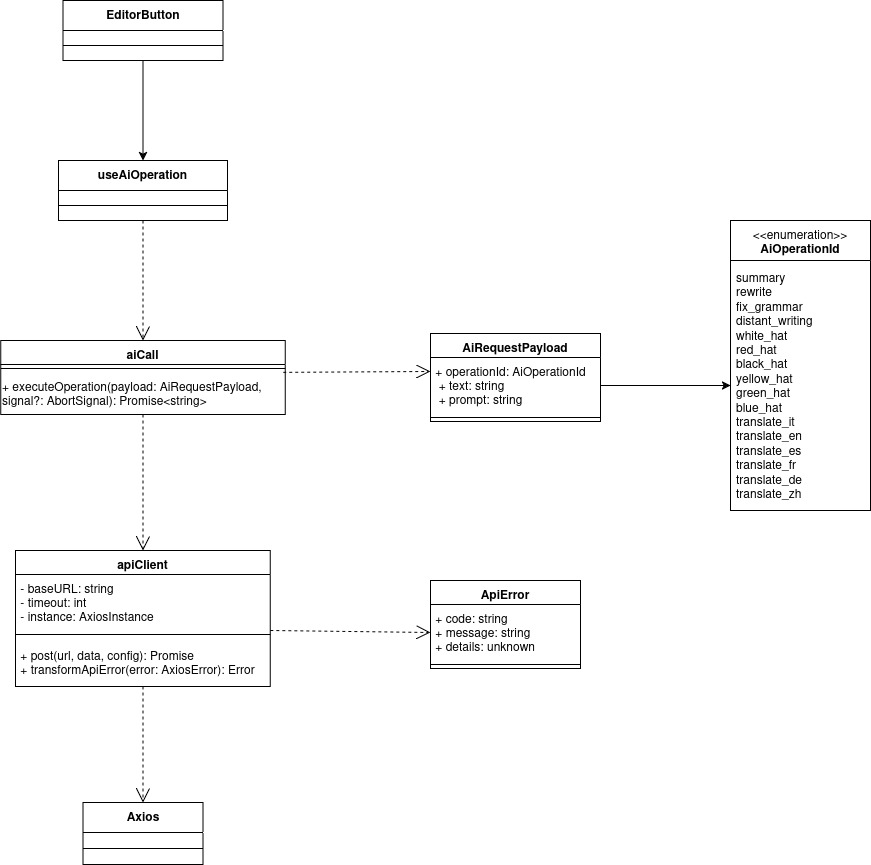
\includegraphics[width=1\textwidth]{../UMLimg/facade.jpg}
    \caption{UML del pattern Facade}
    \label{fig:uml_facade}
\end{figure}



\newpage

% GESTIONE DEGLI STATI DEI WIDGET
\subsection{Gestione degli stati del widget AI}
La gestione dell'interfaccia utente per il widget AI adotta un implementazione a \textbf{stati}. Questa scelta permette di gestire la complessa variabilità visiva del widget in modo modulare e polimorfico.

\subsubsection{Problema}
L’AI Widget è un componente che espone diverse funzionalità in base allo stato dell’operazione in corso. Ogni operazione attraversa una serie di fasi, rendendo esplicita all’utente la condizione della richiesta. Ad esempio, nel caso di un riassunto, il widget passa da uno stato di caricamento, in cui l'utente attende la risposta e in cui è possibile solo annullare l'operazione, a uno stato di visualizzazione del risultato, che l’utente può inserire, eliminare o rigenerare.

In un ambiente dichiarativo come \gls{React}, adottare questo approccio porterebbe il componente principale a gestire ampi blocchi condizionali (come costrutti \texttt{switch} o \texttt{if/else}) per determinare quale porzione di interfaccia renderizzare, generando codice rigido, frammentato e difficile da testare.

\subsubsection{Soluzione: rendering delegato e stati polimorfi}
Nel sistema implementato, il widget si limita a invocare il metodo di rendering dello stato corrente e le relative funzionalità, senza conoscerne l’effettiva implementazione. Ogni stato non è solo comportamentale, ma anche \textbf{presentazionale}: ciascun oggetto-stato è direttamente responsabile del proprio rendering in \gls{React}. Questo consente al componente \texttt{AiWidget} di agire come un semplice coordinatore passivo.

% diagramma per le classi degli stati
\begin{figure}[H]
    \centering
    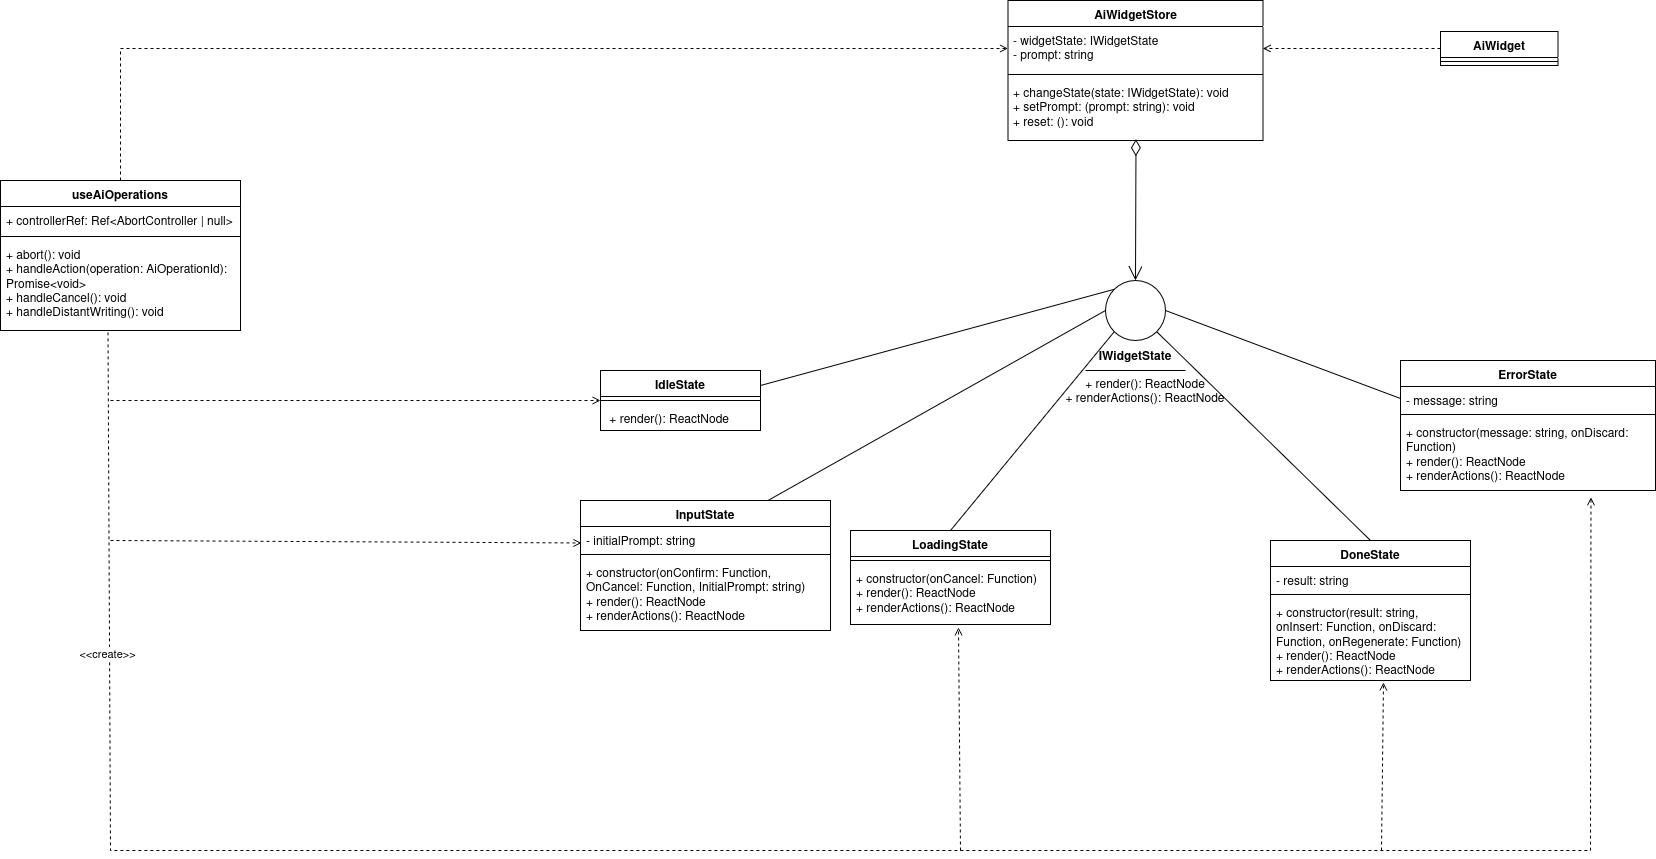
\includegraphics[width=1\textwidth]{../UMLimg/widgetState.jpg}
    \caption{Diagramma delle classi del Render-Delegate State Pattern}
    \label{fig:uml_ai_widget_state}
\end{figure}

\subsubsection{Interfaccia \texttt{IWidgetState}}
Tutti gli stati implementano l'interfaccia comune \texttt{IWidgetState}. Il componente \texttt{AiWidget} non dipende da nessuna delle classi concrete, ma conosce esclusivamente i due metodi definiti dal contratto:
\begin{itemize}
    \item \texttt{render()}: Metodo obbligatorio che produce il contenuto visivo principale del widget.
    \item \texttt{renderActions()}: Metodo opzionale che produce i pulsanti contestuali mostrati nel footer dell'interfaccia.
\end{itemize}

\subsubsection{Classi di stato}
Sono definite cinque classi concrete, ciascuna corrispondente a una fase del ciclo di vita dell'operazione AI:
\begin{itemize}
    \item \textbf{\texttt{IdleState}}: Stato iniziale e di riposo; l'\texttt{AiWidget} non viene renderizzato quando lo stato corrente è un'istanza di questa classe.
    \item \textbf{\texttt{InputState}}: Mostra un'area di testo per l'inserimento del \gls{prompt} da parte dell'utente. Riceve nel costruttore due callback: \texttt{onConfirm} (invocata all'invio) e \texttt{onCancel} (per l'annullamento).
    \item \textbf{\texttt{LoadingState}}: Visualizza un indicatore di caricamento. Accetta opzionalmente una callback \texttt{onCancel} che, se fornita, abilita il pulsante di interruzione della richiesta.
    \item \textbf{\texttt{DoneState}}: Mostra il testo generato e le azioni disponibili: \textit{Inserisci} (inserisce il risultato nell'editor e riporta il widget a \texttt{IdleState}), \textit{Scarta} (riporta il widget a \texttt{IdleState}) e \textit{Rigenera} che, in base all'operazione riporta a \texttt{InputState} con il \gls{prompt} precedente oppure ripete la richiesta con gli stessi parametri.
    \item \textbf{\texttt{ErrorState}}: Visualizza un messaggio d'errore e un pulsante per tornare a \texttt{IdleState}.
\end{itemize}

Le callback iniettate nei costruttori vengono catturate in chiusura al momento della transizione, mantenendo il riferimento al contesto operativo corrente senza che gli stati si conoscano tra loro.


\subsubsection{Orchestrazione: store globale e ViewModel}
La "macchina a stati" polimorfica è orchestrata attraverso la collaborazione tra lo store globale e la logica di business del ViewModel.

\paragraph{Lo store (\texttt{aiWidgetStore})}
Lo stato corrente è mantenuto globalmente in uno store gestito tramite la libreria \textbf{\gls{Zustand}}. Nello store, lo stato non è un parametro primitivo, ma un'istanza diretta dell'interfaccia \texttt{IWidgetState}. Le transizioni avvengono sostituendo integralmente l'istanza tramite la funzione dedicata \texttt{changeState(newState: IWidgetState)}, che innesca l'aggiornamento reattivo dell'interfaccia.\\\\
Lo store si occupa inoltre di mantenere il \textit{\gls{prompt}} relativo all’ultima operazione, in modo da poterlo recuperare facilmente in caso di rigenerazione.

\paragraph{ViewModel (\texttt{useAiOperations})}
L'orchestrazione delle transizioni è centralizzata nel \textit{custom hook} \texttt{useAiOperations}. Questo componente funge da "regista" del pattern:
\begin{itemize}
    \item Istanzia le classi di stato iniettando le callback operative.
    \item Gestisce le chiamate \gls{api} verso il backend.
    \item Gestisce il ciclo di vita dell'\texttt{AbortController} per la cancellazione delle richieste.
\end{itemize}

Il flusso logico principale gestito dal ViewModel è il seguente:
\begin{equation*}
\texttt{Idle} \xrightarrow{\text{avvio operazione}} \texttt{Loading} \xrightarrow{\text{successo}} \texttt{Done} \xrightarrow{\text{inserisci / scarta}} \texttt{Idle}
\end{equation*}

Nel caso dell'operazione \textit{\gls{Distant Writing}}, che richiede un \gls{prompt} esplicito dell'utente, il flusso viene esteso:
\begin{equation*}
\texttt{Idle} \to \texttt{Input} \to \texttt{Loading} \to \texttt{Done} \xrightarrow{\text{rigenera}} \texttt{Input}
\end{equation*}
In entrambi i percorsi, un errore durante la chiamata porta istantaneamente a \texttt{ErrorState}, mentre la cancellazione esplicita da parte dell'utente riporta direttamente a \texttt{IdleState}.

\subsubsection{Separazione delle responsabilità}
Questa architettura garantisce una netta separazione tra rendering e logica: \texttt{AiWidget} è un componente principalmente coordinatore che delega ogni decisione all’oggetto stato corrente; le classi di stato gestiscono la struttura visiva e le callback iniettate, senza contenere logica di business; \texttt{useAiOperations} rappresenta l’unico punto in cui risiedono la logica applicativa, le transizioni di stato e la gestione degli errori.


\newpage

\section{Tracciamento dei requisiti}
In questa sezione è stato riportato il tracciamento dei requisiti del progetto "Second Brain" con lo scopo di avere una panoramica completa sui requisiti stabiliti nel documento dell'\gls{Analisi dei Requisiti} v.2.0.0 e sul loro conseguimento.

\subsection{Notazione dei requisiti}
Il codice identificativo segue il formato:
\[
R[Importanza]-[Tipo]-[Numero]
\]
Dove le voci assumono i seguenti significati:

\begin{description}
    \item[Importanza] \hfill \\
    Indica il grado di priorità del requisito:
    \begin{itemize}
        \item \textbf{O (Obbligatorio):} Requisito esplicitamente richiesto dall'azienda Zucchetti. La sua mancata implementazione implica il fallimento degli obiettivi primari del progetto.
        \item \textbf{D (Desiderabile):} Requisito non strettamente vincolante ma che il gruppo si impegna ad implementare per migliorare il prodotto.
        \item \textbf{OP (Opzionale):} Requisito di priorità minore, la cui implementazione può essere rimandata.
    \end{itemize}
    
    \item[Tipo] \hfill \\
    Indica la natura del requisito:
    \begin{itemize}
        \item \textbf{F (Funzionale):} Descrive le funzionalità e i servizi che il sistema deve fornire.
        \item \textbf{V (Vincolo):} Descrive limitazioni tecnologiche, normative o implementative imposte esternamente.
        \item \textbf{Q (Qualità):} Descrive le caratteristiche qualitative del sistema (es. performance, sicurezza, manutenibilità).
    \end{itemize}
    
    \item[Numero] \hfill \\
    Un numero intero progressivo univoco per tipologia di requisito.
\end{description}

\subsection{Tracciamento dei requisti funzionali}
\begin{longtable}{|c|p{11cm}|c|}
\hline
\textbf{Codice} & \textbf{Descrizione} & \textbf{Stato}\\
\hline
\endhead
RO-F-1 & Il sistema deve fornire un’area di testo per l’inserimento e la modifica del testo con supporto alla sintassi \gls{Markdown} standard (CommonMark). & Soddisfatto \\
\hline
RO-F-2 & Il sistema deve informare l’utente con un messaggio in caso di perdita della connessione Internet durante l’utilizzo dell’editor. & Soddisfatto \\
\hline
RO-F-3 & L'editor deve compilare la sintassi \gls{Markdown} in tempo reale. & Soddisfatto \\
\hline
RO-F-4 & Deve essere presente un'area di visualizzazione del documento formattato rispetto alla sintassi \gls{Markdown}. & Soddisfatto \\
\hline
RO-F-5 & Il sistema deve permettere all'utente di selezionare porzioni di testo tramite mouse o tastiera. & Soddisfatto \\
\hline
RO-F-6 & Il sistema deve permettere all'utente di modificare porzioni di testo selezionate. & Soddisfatto \\
\hline
RO-F-7 & Il sistema deve permettere all'utente di copiare una parte di testo selezionato. & Soddisfatto \\
\hline
RO-F-8 & Il sistema deve permettere all'utente di incollare un testo nell'area di testo. & Soddisfatto \\
\hline
RO-F-9 & Il sistema deve permettere all'utente di tagliare il testo selezionato. & Soddisfatto \\
\hline
RO-F-10 & Il sistema deve permettere all'utente di annullare l'ultima modifica effettuata. & Soddisfatto \\
\hline
RO-F-11 & Se non sono presenti operazioni annullabili, il sistema non esegue alcuna azione al comando Undo. & Soddisfatto \\
\hline
RO-F-12 & Il sistema deve permettere all'utente di ripristinare le modifiche precedentemente annullate. & Soddisfatto \\
\hline
RO-F-13 & Se non sono presenti operazioni ripristinabili, il sistema non esegue alcuna azione al comando Redo. & Soddisfatto \\
\hline
RO-F-14 & Nell'editor deve essere presente una barra degli strumenti (\gls{toolbar}) per applicare formattazioni \gls{Markdown} senza scrivere manualmente la sintassi. & Soddisfatto \\
\hline
RO-F-15 & Il sistema deve permettere l'applicazione del grassetto al testo tramite \gls{toolbar}. & Soddisfatto \\
\hline
RO-F-16 & Il sistema deve permettere l'applicazione del corsivo al testo tramite \gls{toolbar}. & Soddisfatto \\
\hline
RO-F-17 & Il sistema deve permettere l'applicazione della sottolineatura al testo tramite \gls{toolbar}. & Soddisfatto \\
\hline
RO-F-18 & Il sistema deve permettere di creare intestazioni tramite \gls{toolbar}. & Soddisfatto \\
\hline
RO-F-19 & Il sistema deve permettere l'inserimento di elementi di struttura (tabelle, separatori orizzontali) tramite \gls{toolbar}. & Soddisfatto \\
\hline
RO-F-20 & Il sistema deve permettere l'inserimento di liste numerate tramite \gls{toolbar}. & Soddisfatto \\
\hline
RO-F-21 & Il sistema deve permettere l'inserimento di elenchi puntati tramite \gls{toolbar}. & Soddisfatto \\
\hline
RO-F-22 & Il sistema deve permettere l'inserimento di link e riferimenti tramite \gls{toolbar}. & Soddisfatto \\
\hline
RO-F-23 & L'utente può applicare più stili contemporaneamente (es. grassetto, corsivo, sottolineatura) alla stessa sezione di testo. & Soddisfatto \\
\hline
RO-F-24 & L'utente può annullare una formattazione di una porzione di testo selezionato riapplicandola dalla \gls{toolbar}. & Soddisfatto \\
\hline
RO-F-25 & L'utente può estendere la formattazione a una porzione di testo parzialmente formattato riapplicandola dalla \gls{toolbar}. & Soddisfatto \\
\hline
RO-F-26 & L'utente può creare sottoliste attivando la creazione di una lista dalla \gls{toolbar} quando il cursore è già all'interno di una lista. & Soddisfatto \\
\hline
RO-F-27 & L'utente può scegliere una combinazione di formattazioni dalla \gls{toolbar} quando non è presente testo selezionato, per applicarle al testo che scriverà successivamente. & Soddisfatto \\
\hline
RO-F-28 & Il sistema deve permettere all'utente di selezionare porzioni di testo da inviare all'agente esterno. & Soddisfatto \\
\hline
RO-F-29 & Il sistema permette di inviare del testo ad un agente esterno. & Soddisfatto \\
\hline
RO-F-30 & L'utente deve poter accedere alle azioni sul testo tramite agente esterno in ogni momento. & Soddisfatto \\
\hline
RO-F-31 & Il testo generato viene prima mostrato come proposta, separata visivamente dal testo dell'utente. & Soddisfatto \\
\hline
RO-F-32 & Il testo in stato di proposta include le opzioni di conferma, annullamento e rigenerazione. & Soddisfatto \\
\hline
RO-F-33 & Il sistema non permette la modifica del testo generato mentre è in stato di proposta. & Soddisfatto \\
\hline
RO-F-34 & Il testo generato dall'agente esterno, una volta confermato, viene inserito nella posizione del cursore se presente, altrimenti in fondo al testo. & Soddisfatto \\
\hline
RO-F-35 & Una proposta che viene confermata viene inserita nel documento nell'editor e la sezione di proposta viene rimossa. & Soddisfatto \\
\hline
RO-F-36 & Una volta generato e confermato, il testo dell'agente esterno è modificabile tramite le stesse funzionalità dell'editor disponibili per il testo utente. & Soddisfatto \\
\hline
RO-F-37 & Una proposta annullata comporta la rimozione del testo generato dalla sezione di proposta e la rimozione della sezione stessa. & Soddisfatto \\
\hline
RO-F-38 & Una proposta che viene rigenerata viene rimandata all'agente esterno con gli stessi parametri e la nuova risposta sovrascrive la proposta corrente. & Soddisfatto \\
\hline
RO-F-39 & Il sistema deve informare l'utente con un messaggio in caso di errore durante la comunicazione con il servizio LLM. & Soddisfatto \\
\hline
RO-F-40 & L'utente può annullare un'operazione AI in corso prima del suo completamento. & Soddisfatto \\
\hline
RO-F-41 & In seguito all'annullamento di un'operazione AI, il documento rimane nello stato precedente alla richiesta. & Soddisfatto \\
\hline
RO-F-42 & Se la generazione di testo si blocca prematuramente, rimane ciò che è già stato generato, in attesa che l'utente confermi, rigeneri o elimini la proposta. & Soddisfatto \\
\hline
RO-F-43 & L'agente esterno applica modifiche esclusivamente al testo selezionato dall'utente. Un contesto aggiuntivo può essere fornito solo a scopo interpretativo e non deve essere alterato. & Soddisfatto \\
\hline
RO-F-44 & L'utente può consultare il registro delle generazioni AI effettuate. & Soddisfatto \\
\hline
RO-F-45 & Il sistema deve gestire il caso in cui lo storico delle generazioni AI sia vuoto, informando l'utente con un messaggio appropriato. & Soddisfatto \\
\hline
RO-F-46 & Ogni generazione di testo dell'agente esterno viene inclusa nel registro delle generazioni, incluse quelle annullate dall'utente. & Soddisfatto \\
\hline
RO-F-47 & Il sistema deve permettere all'utente di visualizzare il testo completo di una generazione dallo storico AI. & Soddisfatto \\
\hline
RO-F-48 & L'utente deve poter riassumere tutto o una parte selezionata del testo usando un agente esterno. & Soddisfatto \\
\hline
RO-F-49 & L'utente deve poter usare un agente esterno per riscrivere tutto o una parte selezionata del testo migliorandolo seguendo determinate specifiche come sintassi, stile e chiarezza. & Soddisfatto \\
\hline
RO-F-50 & L'utente deve poter tradurre il testo usando un agente esterno in: inglese, italiano, tedesco, francese, spagnolo e cinese mandarino. & Soddisfatto \\
\hline
RO-F-51 & Se l'utente avvia una traduzione senza selezionare la lingua di destinazione, il sistema lo notifica e blocca l'operazione. & Soddisfatto \\
\hline
RO-F-52 & Il sistema permette di avviare la correzione grammaticale del testo tramite agente esterno. & Soddisfatto \\
\hline
RO-F-53 & Se non vengono rilevati errori grammaticali, il sistema informa l'utente dell'esito positivo della correzione. & Soddisfatto \\
\hline
RO-F-54 & Il sistema consente all'utente di avviare l'analisi critica del testo selezionato o dell'intero documento utilizzando il cappello di De Bono scelto. & Soddisfatto \\
\hline
RO-F-55 & Se il testo è insufficiente per l'analisi critica, il sistema notifica l'utente e interrompe l'operazione. & Soddisfatto \\
\hline
RO-F-56 & Se l'utente avvia l'analisi critica senza selezionare un cappello di De Bono, il sistema lo notifica e blocca l'operazione. & Soddisfatto \\
\hline
RO-F-57 & Il sistema permette l'invio di un \gls{prompt} scritto dall'utente per la generazione di testo tramite agente esterno. & Soddisfatto \\
\hline
RO-F-58 & Il sistema permette la modifica del \gls{prompt} da inviare all'agente esterno prima dell'invio. & Soddisfatto \\
\hline
RO-F-59 & L'agente esterno può generare testo basandosi su un \gls{prompt} fornitogli dall'utente. & Soddisfatto \\
\hline
RO-F-60 & Se il \gls{prompt} fornito dall'utente è vuoto o incompleto, il sistema notifica l'utente e impedisce l'invio. & Soddisfatto \\
\hline
RO-F-61 & L'utente può caricare un file dal proprio dispositivo all'interno dell'editor. & Soddisfatto \\
\hline
RO-F-62 & Il sistema deve supportare il caricamento di file in formato \gls{Markdown} (\texttt{.md}, \texttt{.\gls{markdown}}) e testo semplice (\texttt{.txt}). & Soddisfatto \\
\hline
RO-F-63 & Il sistema deve supportare il caricamento tramite dialogo di esplorazione file (file picker). & Soddisfatto \\
\hline
RO-F-64 & Prima di procedere con il caricamento di un file, il sistema chiede conferma all'utente. & Soddisfatto \\
\hline
RO-F-65 & Il sistema deve informare l'utente con un messaggio di esito (successo o errore) al termine di ogni tentativo di caricamento file. & Soddisfatto \\
\hline
RO-F-66 & Il sistema deve validare il formato del file selezionato e impedire il caricamento di formati non supportati. & Soddisfatto \\
\hline
RO-F-67 & Il sistema deve validare le dimensioni del file selezionato e impedire il caricamento di file che superano la dimensione massima consentita. & Soddisfatto \\
\hline
RO-F-68 & Il sistema deve impedire il caricamento di file corrotti o illeggibili. & Soddisfatto \\
\hline
RO-F-69 & Il sistema deve permettere all'utente di rimuovere il file che ha caricato. & Soddisfatto \\
\hline
RO-F-70 & L'utente può annullare l'operazione di rimozione del file caricato, lasciando l'editor nel suo stato precedente. & Soddisfatto \\
\hline
RO-F-71 & Il sistema deve essere in grado di convertire il documento da \gls{Markdown} al formato selezionato dall'utente. & Soddisfatto \\
\hline
RO-F-72 & Il sistema deve permettere di scaricare il file nel dispositivo dell'utente. & Soddisfatto \\
\hline
RO-F-73 & L'operazione di esportazione o stampa non deve alterare né chiudere il documento originale nell'editor. & Soddisfatto \\
\hline
RO-F-74 & Il sistema deve informare l'utente con un messaggio di esito al termine di ogni operazione di esportazione. & Soddisfatto \\
\hline
RO-F-75 & Il sistema deve consentire l'esportazione del documento in formato \gls{Markdown} (\texttt{.md}). & Soddisfatto \\
\hline
RO-F-76 & Il sistema deve controllare che il range di pagine inserito dall'utente sia valido (non superiore al numero di pagine del documento e non negativo). & Soddisfatto \\
\hline
RO-F-77 & Il sistema deve permettere di collegare e inviare il documento a un dispositivo di stampa. & Soddisfatto \\
\hline
RO-F-78 & Il sistema deve informare l'utente con un messaggio in caso di errore durante l'invio del documento alla stampante. & Soddisfatto \\
\hline
RO-F-79 & Il sistema deve garantire la persistenza locale del testo nell'editor tramite browser storage (LocalStorage). & Soddisfatto \\
\hline
RO-F-80 & Il sistema deve garantire la persistenza locale dello storico delle generazioni AI tramite browser storage (\gls{Zustand} persist). & Soddisfatto \\
\hline
RO-F-81 & Il sistema deve impedire il caricamento di file di dimensioni superiori a 5MB. & Soddisfatto \\
\hline

% DESIDERABILI
RD-F-1 & Il sistema deve supportare l'uso di scorciatoie da tastiera per le operazioni di formattazione. & Soddisfatto \\
\hline
RD-F-2 & Il sistema deve permettere di cambiare modalità di visualizzazione (Solo Editor, Solo Anteprima, Split View). & Soddisfatto \\
\hline
RD-F-3 & Il sistema deve supportare il caricamento tramite drag-and-drop (trascinamento file nell'area dell'editor). & Soddisfatto \\
\hline
RD-F-4 & Se sono presenti modifiche non salvate, il sistema chiede conferma all'utente prima di caricare un nuovo file. & Soddisfatto\\
\hline
RD-F-5 & Il parsing del contenuto del file caricato deve gestire caratteri non validi senza causare il crash dell'applicazione. & Soddisfatto \\
\hline
RD-F-6 & I messaggi di errore relativi al caricamento file devono essere esplicativi e suggerire come procedere. & Soddisfatto \\
\hline
RD-F-7 & Il sistema deve offrire più opzioni per le operazioni comuni sui file come carica nuovo, stampa, chiudi. & Soddisfatto \\
\hline
RD-F-8 & Il sistema deve consentire l'esportazione del documento in formato PDF. & Non soddisfatto \\
\hline
RD-F-9 & Il sistema deve consentire l'esportazione del documento in formato HTML. & Soddisfatto \\
\hline
RD-F-10 & Il sistema deve consentire l'esportazione del documento in formato ODT. & Non soddisfatto \\
\hline
RD-F-11 & Il sistema deve consentire l'esportazione del documento in formato DOCX. & Non soddisfatto \\
\hline
RD-F-12 & L'utente deve poter scegliere se esportare l'intero documento o un range di pagine selezionate. & Non soddisfatto \\
\hline
RD-F-13 & Il sistema deve consentire all'utente di scegliere il nome del file prima di procedere al download/esportazione. & Soddisfatto \\
\hline
RD-F-14 & Il sistema deve fornire un'anteprima del documento nel formato selezionato prima di procedere al download. & Non soddisfatto \\
\hline
RD-F-15 & Il sistema deve aprire il dialogo di stampa nativo del browser per configurare le opzioni di stampa. & Soddisfatto \\
\hline
RD-F-16 & Il sistema deve informare l'utente con un messaggio se l'editor non risponde ai comandi. & Non soddisfatto\\
\hline
RD-F-17 & Il sistema deve informare l'utente con un messaggio se il pannello di anteprima non si aggiorna correttamente. & Non soddisfatto \\
\hline

% OPZIONALI
ROP-F-1 & L'utente può ricercare parole nel testo attraverso l'editor & Non soddisfatto \\
\hline
ROP-F-2 & Il sistema deve informare l'utente se la ricerca non ha prodotto occorrenze nel testo. & Non soddisfatto \\
\hline
ROP-F-3 & La sezione di testo generata come proposta è visibilmente diversa dal testo utente & Soddisfatto \\
\hline
ROP-F-4 & Per ogni voce del registro delle generazioni AI il sistema deve indicare la data e l'ora della generazione. & Soddisfatto \\
\hline
ROP-F-5 & Per ogni voce del registro delle generazioni AI il sistema deve indicare il tipo di operazione che ha prodotto la generazione. & Soddisfatto \\
\hline
ROP-F-6 & L'utente può eliminare una voce dal registro delle generazioni AI. & Soddisfatto \\
\hline
ROP-F-7 & Per gli utenti autenticati, il registro delle generazioni AI è persistente ed è associato ai documenti salvati nel proprio account. & Non soddisfatto \\
\hline
ROP-F-8 & La sezione di testo in stato di proposta viene colorata in base al tipo di operazione che viene fatta & Soddisfatto \\
\hline
ROP-F-9 & Il sistema deve visualizzare sia il testo originale che la traduzione generata, permettendo all'utente di confrontarle. & Soddisfatto \\
\hline
ROP-F-10 & Se il testo selezionato è già nella lingua di destinazione della traduzione, il sistema avvisa l'utente e interrompe l'operazione. & Non soddisfatto \\
\hline
ROP-F-11 & Il sistema offre esempi per la richiesta di generazione di testo a partire da un estratto & Non soddisfatto \\
\hline
ROP-F-12 & Il sistema permette di inserire un grafico generato, con dati presenti nel testo, scelto tra diversi tipi disponibili all'utente & Non soddisfatto \\
\hline
ROP-F-13 & Il sistema permette di inserire una tabella generata con dati presenti nel testo & Non soddisfatto \\
\hline
ROP-F-14 & Se i dati nel testo sono insufficienti per generare grafici o tabelle, il sistema notifica l'utente. & Non soddisfatto \\
\hline
ROP-F-15 & Il sistema permette di inserire una mappa concettuale generata con dati presenti nel testo & Non soddisfatto \\
\hline
ROP-F-16 & Se si verificano errori nella visualizzazione della mappa concettuale generata, il sistema notifica l'utente. & Non soddisfatto \\
\hline
ROP-F-17 & Il sistema permette di inserire una formula matematica generata con dati presenti nel testo & Non soddisfatto \\
\hline
ROP-F-18 & Se la formula matematica contiene simboli non supportati, il sistema notifica l'utente. & Non soddisfatto \\
\hline
ROP-F-19 & Il sistema deve permettere all'utente di inserire le proprie credenziali (username e password) per il login & Non soddisfatto \\
\hline
ROP-F-20 & Se le credenziali sono errate il sistema non permette all'utente di autenticarsi & Non soddisfatto \\
\hline
ROP-F-21 & Il sistema deve mostrare un messaggio di errore generico in caso di fallimento del login, senza specificare se l'errore riguarda username o password. & Non soddisfatto \\
\hline
ROP-F-22 & In caso di username già esistente durante la registrazione, il sistema deve proporre all'utente di effettuare il login o scegliere un nuovo username. & Non soddisfatto\\
\hline
ROP-F-23 & Il sistema deve permettere all'utente di potersi registrare tramite uno username e una password & Non soddisfatto \\
\hline
ROP-F-24 & Il sistema deve impedire la registrazione in caso ci sia uno username uguale nel \gls{database} & Non soddisfatto\\
\hline
ROP-F-25 & Il sistema deve salvare nel \gls{database} le password criptate in fase di registrazione & Non soddisfatto \\
\hline
ROP-F-26 & Il sistema deve permettere ad un \gls{utente autenticato} di poter eliminare il proprio account & Non soddisfatto \\
\hline
ROP-F-27 & Il sistema in caso di eliminazione account deve eliminare i dati dal \gls{database} & Non soddisfatto \\
\hline
ROP-F-28 & Le operazioni di eliminazione dell'account devono richiedere una conferma esplicita da parte dell'utente & Non soddisfatto \\
\hline
ROP-F-29 & Il sistema deve terminare la sessione se un account viene eliminato & Non soddisfatto \\
\hline
ROP-F-30 & L'utente può annullare la procedura di eliminazione del proprio account. & Non soddisfatto \\
\hline
ROP-F-31 & Il sistema deve permettere ad un utente di vedere i file che ha salvato & Non soddisfatto \\
\hline
ROP-F-32 & Il sistema deve permettere ad un \gls{utente autenticato} di selezionare un file dall'elenco di quelli salvati e aprirlo & Non soddisfatto \\
\hline
ROP-F-33 & Il sistema deve permettere all'utente di annullare l'operazione di apertura file, lasciando l'editor nel suo stato precedente. & Soddisfatto \\
\hline
ROP-F-34 & Il sistema deve mostrare i file salvati in ordine cronologico per data di ultima modifica. & Non soddisfatto \\
\hline
ROP-F-35 & L'accesso ai file salvati nel \gls{database} è consentito solo ad utenti autenticati. & Non soddisfatto \\
\hline
ROP-F-36 & Il sistema deve permettere il salvataggio di un file in un \gls{sistema di persistenza} non locale & Non soddisfatto \\
\hline
ROP-F-37 & Il sistema deve notificare l'utente in caso di fallimento del salvataggio nel \gls{database}. & Non soddisfatto \\
\hline
ROP-F-38 & Il sistema deve associare ogni file al suo creatore & Non soddisfatto \\
\hline
ROP-F-39 & Il sistema deve impedire il salvataggio di file nel \gls{database} da parte di utenti non autenticati. & Non soddisfatto \\
\hline
ROP-F-40 & Il sistema deve impedire il salvataggio di un documento vuoto nel \gls{database}. & Non soddisfatto \\
\hline
ROP-F-41 & Un \gls{utente non autenticato} che prova a salvare un file viene riportato alla pagina di login & Non soddisfatto \\
\hline
ROP-F-42 & L'utente può effettuare il logout in ogni momento e terminare la propria sessione & Non soddisfatto \\
\hline
ROP-F-43 & Il sistema deve permettere all'utente di modificare il nome del documento corrente direttamente dall'interfaccia di lavoro. & Soddisfatto \\
\hline
ROP-F-44 & Il sistema deve permettere all'utente di cercare testo all'interno del registro delle generazioni AI tramite una barra di ricerca. & Soddisfatto\\
\hline
ROP-F-45 & Il sistema deve permettere all'utente di filtrare le voci del registro delle generazioni AI in base al tipo di operazione effettuata. & Soddisfatto\\
\hline
\addlinespace[1em]
\caption{Tracciamento dei \gls{requisiti funzionali}}
\label{tab:tracciamento_requisiti_funzionali}
\end{longtable}

\subsection{Tracciamento dei requisti di qualità}
\begin{longtable}{|c|p{11cm}|c|}
\hline
\textbf{Codice} & \textbf{Descrizione} & \textbf{Stato}\\
\hline
\endhead
RO-Q-1 & Il tempo di risposta dell'interfaccia utente (aggiornamento anteprima, applicazione formattazioni) deve essere inferiore a 500 ms nel 95\% dei casi, misurato su una sessione utente attiva di almeno 30 minuti. & Soddisfatto \\
\hline
RO-Q-2 & Il tempo medio di generazione di una risposta da parte del servizio LLM non deve superare i 30 secondi, misurato su un campione di almeno 20 richieste consecutive in condizioni di utilizzo normale.  & Soddisfatto \\
\hline
RO-Q-3 & Il tasso di errori nelle operazioni principali (salvataggio, apertura file, chiamate AI) non deve superare l'1\%, misurato sul totale delle operazioni eseguite in una sessione utente attiva di almeno 30 minuti. & Soddisfatto \\
\hline
RO-Q-4 & La percentuale di codice coperta dai test automatici (test coverage) deve essere almeno il 70\%, misurata sull'insieme completo dei moduli rilasciati ad ogni versione. & Soddisfatto \\
\hline
RO-Q-5 & La complessità ciclomatica (McCabe) di ogni funzione/metodo del codice prodotto non deve superare il valore 8. & Soddisfatto \\
\hline
RO-Q-6 & La documentazione prodotta deve ottenere un Indice di Gulpease (IG) maggiore o uguale a 40. & Soddisfatto \\
\hline
RO-Q-7 & Il sistema deve essere sviluppato rispettando le Norme 
di Progetto del gruppo ByteMe. & Soddisfatto \\
\hline
RO-Q-8 & Il sistema deve essere verificato secondo il Piano di Qualifica prima di ogni rilascio. & Soddisfatto\\
\hline
RO-Q-9 & Il \gls{manuale utente} deve documentare tutte le funzionalità obbligatorie del sistema e deve ottenere un Indice di Gulpease (IG) maggiore o uguale a 40. & Soddisfatto \\
\hline
RO-Q-10 & Il manuale di installazione e deployment del sistema deve ottenere un Indice di Gulpease (IG) maggiore o uguale a 40. & Soddisfatto \\
\hline
\addlinespace[1em]
\caption{Tracciamento dei \gls{requisiti di qualità}}
\label{tab:tracciamento_requisiti_qualità}
\end{longtable}

\subsection{Tracciamento dei requisti di vincolo}
\begin{longtable}{|c|p{11cm}|c|}
\hline
\textbf{Codice} & \textbf{Descrizione} & \textbf{Stato}\\
\hline
\endhead
RO-V-1 & L'applicazione deve essere accessibile tramite browser web. 
I browser supportati sono: Google Chrome ($\geq$ v110), Mozilla Firefox 
($\geq$ v110), Microsoft Edge ($\geq$ v110), Safari ($\geq$ v16). & Soddisfatto \\
\hline
RO-V-2 & Il sistema deve utilizzare la codifica Unicode (UTF-8) per la rappresentazione interna e lo storage del testo. & Soddisfatto \\
\hline
RO-V-3 & Il formato di input e di storage del testo deve essere \gls{Markdown}, in conformità allo standard CommonMark. & Soddisfatto\\
\hline
RO-V-4 & Il sistema deve integrarsi con un servizio LLM tramite \gls{API} REST compatibili con lo standard OpenAI. & Soddisfatto \\
\hline
\addlinespace[1em]
\caption{Tracciamento dei \gls{requisiti di vincolo}}
\label{tab:tracciamento_requisiti_vincolo}
\end{longtable}

\end{document}